%Copyright (C) 2021-2023 Geoff Beck. This work is licensed under a Creative Commons Attribution-ShareAlike 4.0 License. To view a copy of this license visit: \url{https://creativecommons.org/licenses/by-sa/4.0/legalcode


\documentclass[a4paper,10pt,oneside]{book}

\usepackage{fullpage,appendix}
\usepackage{amsmath}
\usepackage{import,url}
\usepackage{tocbibind}
\usepackage[bookmarks=true,plainpages=false]{hyperref}
\usepackage{titletoc}
\usepackage{graphicx}
\usepackage{caption,titlecaps}
\usepackage[a4paper,margin=2cm]{geometry}

\graphicspath{{pictures/}}
\usepackage[T1]{fontenc}
\usepackage{lmodern}


\usepackage{fancyhdr}
\usepackage{titling}
\title{\textbf{\huge Heroes3D6\\Core rules}}
\author{Geoff Beck}
\predate{\centering}
\date{}
\postdate{\vfill{\copyright 2021-2023 Geoff Beck. This work is licensed under a Creative Commons Attribution-ShareAlike 4.0 License. To view a copy of this license visit: \url{https://creativecommons.org/licenses/by-sa/4.0/legalcode}}\hfill}
\usepackage{lipsum}
\pagestyle{plain}


\newcommand{\dicediffbase}{9}
\newcommand{\dicecritlvl}{3}

\newcommand{\textlf}[1]{\textbf{\titlecap{#1}}}
\newcommand{\textlfirst}[1]{\textbf{\textit{\titlecap{#1}}}}



\begin{document}
\frontmatter
\maketitle
\tableofcontents
\mainmatter

\chapter{Introduction}

\section{Opening words}
A player's character is their representative in the world of \textit{Heroes3D6} and such should be a personal and fully customisable thing; allowing the player's creativity free reign and not limiting them with too many rules and class attributes etc. This is what \textit{Heroes3D6} tries to do, liberate your role playing experience from restrictive parameters but still maintain some semblance of an ordered and enjoyable system.

\textit{Heroes3D6} depends almost as much on the imagination of the players as it does upon the Game Master. The players are given little or no instruction as to how to fulfil any role within a group and how well they do this will ultimately decide how much fun the game is.

This is a simple system to pick up, as it applies a central set of mechanics across the board, but is complicated enough to please even the most hardcore of gamers, due to the depth and freedom of its mechanics, should you choose to delve into them. The system itself is very open to interpretation and lots of work is required by the Game Master to make this work, as they must make many decisions on the spot as to how the rules apply in a given situation. Other than that, just read and play.

This weighty tome encompasses all the essential rules needed to play a game of \textit{Heroes3D6} independent of setting, other books merely contain rules for playing the game within a famous/iconic world or setting, all these other books require these Core Rules, but do occasionally over-ride them when necessary.

\section{The core system}
\label{sec:base}

\subsection{Players and the game master (GM)}
Games of Heroes are run by a player designated as the Game Master (GM). The remaining participants are simply termed as players. Each of the players controls a character and together they will take part in an adventure supervised by the GM. The Game Master acts as a narrator, they drive the story and is in control of the world and environments inhabited by the player characters. Additionally, they create and control any people or monsters that the characters will encounter in the course of their adventures. 

These rules for the structure of the game are deliberately loose, as the freedom of players and GM to collectively shape an adventure is the magic that makes pen-and-paper role-playing games worthwhile.

\subsection{Actions and dice rolls}
An element of randomisation is introduced into the game by the players rolling dice whenever their characters wish to perform non-trivial actions. These rolls tend to be modified by how good the character is at the particular action (making them more or less likely to succeed). Things like breaking down doors, persuading a guard to let you into a locked door, picking a lock, fighting an enemy, noticing someone hiding in the bushes, climbing a tree/wall/ladder/rope, swimming, jumping a gap, riding, or picking pockets are all examples of actions that would require the player to make a roll to see if their character succeeds. Because the system is based on rolling 3 six-sided dice, the resulting non-linear probability distribution means we can also decide upon the degree of success in a manner that is far more realistic than one resulting from rolling a single dice. 

How good a character is at a particular action is decided by two things, firstly their natural capabilities (Chapter~\ref{chap:attb}) and secondly their learned or acquired skills (Chapter~\ref{chap:skills}). Deciding whether or not a skill or natural attribute is appropriate to a particular task is a matter of common sense and the players and GM can come to a consensus for any contentious tasks. For example: tasks that rely only on the characters strength (actions like breaking things) will not be resolved through skills. However, actions like riding horses, tying or climbing ropes, and picking locks are all things that are greatly enhanced by experience and thus will depend on more than just the character's raw personal ability when resolving such actions.  

How success and failure are determined is explained in the Section~\ref{sec:rolls} below.

\subsubsection{Dice notation}
The notation ``requires a 3d6 roll of $16+$'' means that a total score of 16 or greater, on three six-sided dice (3d6), is needed for the given action to succeed. Similarly ``$5-$'' means 5 or less. When no dice code (3d6, 2d6, etc) is given, then 3d6 is considered the default dice set.

\subsubsection{Opposed rolls and difficulty checks}
\label{sec:rolls}
The core of this 3d6 system is the \textlfirst{difficulty check}, any task can be assigned a \textlfirst{difficulty} by the Game Master and then is performed successfully if the character scores equal to or greater than the \textlf{difficulty} on a roll of 3d6. To this roll you add the relevant \textlfirst{attribute} score; for instance when making a climbing check you add your \textlf{Might} score to the roll. The second core mechanic is the \textlfirst{opposed roll}, this represents a contest between two or more opponents, as such each creature contesting the roll adds the given \textlf{attribute} score to a roll of 3d6. The victor is the one whose resultant score is the highest. In the case of a tie, the tied parties simply roll again.

\subsubsection{Critical success/failure}
If you succeed/fail on a check by $\dicecritlvl$ or more you have achieved a \textlfirst{critical success/failure}. For example, if you need to beat \textlf{difficulty} 11 to succeed, then $14+$ is \textlf{critical success} whereas $8-$ is \textlf{critical failure}. Some effects scale with how many multiples of $\dicecritlvl$ you succeed or fail by.

\subsubsection{Rounding conventions}
When the division of an integer score results in a non-integer number (i.e. $7.5$ or $9.1$) then the convention is to round up, unless otherwise specified.

\subsubsection{Edge}
Some circumstances confer great advantage or disadvantage on a character. This is referred to as having an \textlfirst{edge}. When rolling 3d6 with an \textlf{edge} bonus (\textlf{edge+}), a character rolls 4d6 and chooses the highest 3. In contrast, an \textlf{edge} penalty (\textlf{edge-}) makes the character roll 4d6 dice and choose the lowest 3. Example: I roll 3d6 to make a check to see if I jump over a crevasse, luckily I have \textlf{edge+} and thus roll 4d6 scoring 3,4,2, and 3. I keep the highest 3 and total 10. If this was \textlf{edge-} I would have totalled 8. 

\textlf{edge-} cancels out \textlf{edge+} if character is subject to both, e.g. if your character is suffering two \textlf{edge} penalties but has one bonus, they are effectively experience \textlf{edge-}. If a character has 2 or more \textlf{edge} bonuses/penalties simply add extra dice to the number being rolled, i.e. \textlf{edge++} means a 3d6 roll becomes 5d6 and choose the best 3. The general pattern is: when rolling $n$d6 and having $m$ \textlf{edge} bonuses/penalties, you instead roll $(n+m)$d6 and choose the highest/lowest $n$ dice. 

\subsection{Heroic statistics}
Any heroic/villainous character will also posses an attribute called \textlfirst{heroism/villainy}, which can be spent to perform feats of exceptional skill and daring. The central premise of this statistic system is to set heroic characters apart, allowing them to occasionally avoid the vagaries of chance inherent in dice rolling games. 


\section{Useful notes for the GM}
Here we will discuss an important topic: how we assign \textlf{difficulty} scores to feats characters wish to perform. This is non-trivial if you are used to systems that use a single die for rolls, i.e. 1d20 being rolled for skill checks etc. 

\subsection{Assigning difficulties}
The trickiness of \textlf{difficulty} assignment arises from the fact that 3d6 have a non-linear probability distribution, meaning that some scores are far more likely than others. Whereas, on 1d20 every score has an equal chance of occurring. Thus, the GM should be careful, as an increase of 1 \textlf{difficulty} can make a task far more difficult than you would anticipate. To help with this task, I will outline some useful principles in choosing difficulties. The very nerdy reader can look to the appendices for fun things like probability distributions. 

I will divide tasks into 3 groups: easy, moderate, and hard. In order to view these in a vaguely concrete framework, I will sort \textlf{difficulty} scores into these groups assuming there are no bonuses or penalties on the roll. In this situation, a \textlf{difficulty} of lower than 9 is easy, and greater than 13 is rather hard. 

Note that requiring $11+$ on 3d6 is a 50\% probability of success, so this would correspond to something an unskilled character is equally likely to fail or succeed at. A \textlf{difficulty} of $13$ would only imply success 25\% of the time (assuming no bonuses). In contrast, a \textlf{difficulty} of $9$ results in a chance of 75\% of succeeding. These examples should give you sufficient idea of how to assign \textlf{difficulty}. Things that an average man would struggle to achieve should be \textlf{difficulty} $13$ or higher whereas simple tasks can assigned $9$ or lower. In this $9$ to $13$ range each increase or decrease in \textlf{difficulty} by $1$ results in the same probability shift, for lower or higher difficulties the distribution becomes more extreme.




\chapter{Character attributes}
\label{chap:attb}

A character in \textit{Heroes3D6} is represented by a set of \textlfirst{natural attributes} and their \textlf{heroism/villainy}. The former detail the character's innate abilities while the latter represent their calibre as a potential hero or villain.
Natural attributes are: \textlfirst{might}, \textlfirst{cunning}, \textlfirst{wit}, and \textlfirst{resolve}.

Natural attributes can be used to determine a character's success in certain actions (examples are given in the sections below). As such, success is determined by making a \textlf{difficulty check} with the given attribute.

\section{Natural attributes}
These reflect the inherent predispositions of the character, based on their personality. There are four attribute statistics and a character's scores are determined following the character creation rules, found in Chapter~\ref{chap:create}. 

\subsection{Attribute modifiers}
Each attribute contributes to many different skills or activities, its influence on dice rolls is direct, just add it to the result of a relevant roll.

\subsection{Might}
\textlf{Might} is the aggression or assertiveness of the character. A character can make might-checks to, through sheer bloody-mindedness, break objects, bash in doors, or move large objects. \textlf{Might} dictates a character's ability to inflict damage in combat, enhances any attempted feats of \textlf{athletics}, and augments their ability to \textlf{intimidate} others.

\subsection{Cunning}
\textlf{Cunning} is the craftiness of the character. \textlf{Cunning} can be used to bluff convincingly, make feints in combat, trip people up, or get out of the way of harm. It also contributes to the \textlf{stealth}, \textlf{disguise}, \textlf{deceive}, \textlf{slight of hand}, and \textlf{survival} skills. 

\subsection{Wit}
\textlf{Wit} is a character's ability to rapidly adjust to changing circumstances. It affects a character's aim in combat as well as the \textlf{awareness}, \textlf{mechanical}, and \textlf{knowledge} skills. \textlf{Wit} checks would be made if the character had to rapidly assess a situation or react quickly to imminent danger. \textlf{Wit} also decides how difficult it is to deceive or confuse the character. 

\subsection{Resolve}
Is a measure of the character's determination and force of character. \textlf{Resolve} checks can be used to flatter, distract, or to taunt/enrage a target into attacking the character. \textlf{Resolve} is also involved in the \textlf{persuade}, \textlf{leadership}, \textlf{healing}, \textlf{insight}, and \textlf{perform} skills. Finally, it regulates a character's ability to resist debilitating effects (magic,drugs,poisons) by pure will. 



\section{Perks \& proficiencies}

\textlfirst{Perks} are talents learned or gained by a hero through the course of their adventures, they can be purchased via the expenditure of experience points. A character can have at most 3 active and 3 passive \textlf{perks} equipped at once (only equipped \textlf{perks} can be used). A character can make only one change to which \textlf{perks} are equipped each day.

\textlf{Proficiencies} are more general skills gained by the character. These are always in effect and never occupy either passive or active \textlf{perk} equipment slots.
A list of \textlf{perks} and \textlf{proficiencies} can be found in Chapter~\ref{chap:perks}.


\section{Heroic attributes}
\label{sec:heroism}
\subsection{Heroism/Villainy}
\textlf{Heroism} is what sets your character apart from their more ordinary brethren, it represents a hero's capacity to make decisive and daring actions under pressure. The distinction between \textlf{heroism} and \textlf{villainy} points is one of flavour, villains have \textlf{villainy} while heroes get \textlf{heroism}. Generally, if a rule refers to \textlf{heroism} it still pertains to \textlf{villainy}, unless otherwise stated. 

\textlf{Heroism/Villainy} may be spent to raise the success level of a single action by 1 (i.e. a \textlf{critical failure} becomes plain failure, success becomes \textlf{critical success}, and \textlf{critical success} goes to level 2 \textlf{critical success}). Additionally, \textlf{heroism} may be spent to perform daring feats of valour while \textlf{villainy} may be used for vile trickery; this grants the character access to a single \textlf{perk} of their choice for 6 seconds (1 round in combat). There is no need for the character to have bought the chosen \textlf{perk} or have it equipped (it also bypasses limits on \textlf{perk} numbers).

If a character has no \textlf{heroism/villainy} when resting, they may regain 1 point. Otherwise, such points are awarded by the Game Master on the spur of the moment for any deed that is appropriately heroic/villainous. 


\subsubsection{Moment of glory}
A \textlfirst{moment of glory} awards the character with a single \textlf{heroism/villainy} point they can spend within the next round only.

\subsubsection{Optional rules}
An alternative way to use \textlf{heroism} is to allow characters to make special actions they invent on the spot. The Game Master must decide the consequences of any such actions made.



\section{Experience points}
Each time the Game Master decides to reward the heroic achievement of a character, or each character in the group, then the relevant characters gain 1 experience point. 
This guideline is very qualitative and this is because heroism is a qualitative thing, so advancement is very much a case of the application of GM judgement, informed by basic guidelines laid down here. 

Simple guidelines for experience: a point can be earned by actions demonstrating some heroic calibre, such as: single handedly over-coming many foes or performing reckless feats of strength and daring that save the day. Or perhaps by feats of magic or deeds accomplished through strength of will and force of personality. Experience can also be awarded for devious acts of deceit, or from victory through wit and intelligence rather than blade and boot. Note that these achievements are not combat exclusive, heroism is format-independent after all.

Experience points can be spent on purchasing new \textlf{perks} and \textlf{proficiencies}, the costs of these is detailed in Chapter \ref{chap:perks}. Note that experience cannot be spent in high pressure or active situations, only during periods of rest and contemplation. When you purchase a new \textlf{perk} or \textlf{proficiency}, you must spend 2 hours of down-time practising with your new ability before it can be used in any high pressure situation.

\subsection{Advancing attributes}
Natural attribute points can only be increased in a limited fashion, so choose wisely! The only way to do so is via the \textlf{hero/villain} proficiency from Chapter~\ref{chap:perks}.



\section{Reputation}
Any hero or villain has a reputation, be it as a magnanimous defender or a scheming thief; so to can characters develop a reputation and even, by great deeds, have their names known and talked of by thousands of admirers/policemen. 

\subsection{Reputation level}
Reputation is gained by performing important deeds or actions that get you talked about. Saving the mayor's daughter or preventing bandits from robbing a group of farmers, that kind of thing. Cheating lots of people out of their money, swindling a local lord, or even robbing a bank are also good examples of reputation gaining actions.
Each character has a personal reputation, which is that of the group but modified by personal actions, and the group as a whole has a reputation based on group actions.
Characters start at 0 reputation.

\subsection{Reputation rating}
This indicates whether your reputation is good or bad, it starts at 0 normally, but depending on your Game Master, it can start at -1 or +1. If you gain reputation for ``bad'' actions you get -1 reputation rating, ``good'' actions get +1, so a negative reputation makes you infamous while positive makes you well-liked.





\chapter{Making a character}

\label{chap:create}
Simply follow these steps to create a character:
\begin{itemize}
\item
First browse the species available in the campaign setting and choose yourself one, you may wish to select this based on the modifiers applied to members of that group, or simply on a whim. The default human option would allow you to spend an extra 2 points when choosing \textlf{perks} and \textlf{proficiencies} at character creation.
\item
Now create a \textlfirst{background} following Section~\ref{sec:backgrounds}. 
\item 
Select at least one \textlfirst{Conviction} for your character from \ref{sec:convictions} or invent your own.
\item
Come up with the \textlfirst{Flaw} in your character's personality, with examples in Section~\ref{sec:flaws} (you may have two flaws at most).
\item
Decide the \textlfirst{goals} that drive your character to pursue adventure.
\item
What \textlfirst{relationships} link the character to other group members, organisations, or people in their past?
\item
Now we come to the most important part of character creation: deciding what kind of person they are. Use the \textlf{Convictions}, \textlf{flaws} and \textlf{goals} you chose as a skeleton. You need to define a character you are comfortable to play as, but also one who is believable as a real person. Lets face it, its not much of a role playing game if everyone is just a faceless killing machine.
\item
Choose one \textlf{attribute} to have the value 2, and another to have 1. Set all other \textlf{attributes} to 0 (try and make your choices align with the character's personality).  Set \textlf{heroism/villainy} to 1. 
\item 
Select 3 weapon or skill \textlf{proficiencies} (in any combination you choose). Try to match these up to your \textlf{background}.
\item
Spend up to 3 experience points choosing \textlf{perks} (Chapter~\ref{chap:perks}) for your character.  
\item
Now you may select starting equipment, either from a list supplied by the Game Master or from a budget.
\item
Calculate your combat statistics (see Section~\ref{sec:comstat}).
\end{itemize}



\section{Character backgrounds}
\label{sec:backgrounds}
The character's background is their history before adventuring and dictates the set of associated skills they can choose on character creation. To create a background simply decide on your character's past and choose what kind of skills this would make them proficient in. Here we will list a few examples to give you ideas, if you use any of these you should flesh them out and make them more detailed.

\subsection{Soldier}
The character is a hard-bitten veteran of fighting. Having seen their fair share of blood spilt on the orders of others, they now turn their hand to adventuring instead. Soldier encompasses many possible histories. Some examples might be: army conscript, mercenary, city guard, bandit, or gang enforcer. Skill suggestions: Healing, Survival, Ride, Athletics, Leadership. 

\subsection{Guttersnipe}
The character was born into a life of poverty, scrounging, stealing, and fighting for scraps in back-alleys. This background lends itself to producing street-smart characters who grew up in harsh environments. Such a character is used to being on the wrong side of the law, sometimes through no fault of their own. Skill suggestions: Stealth, Slight of hand, Deceive, Insight, Athletics, Awareness.

\subsection{Wanderer}
The character lives the life of a vagrant or vagabond. They move from place to place seeking opportunity, profit, or just thrills. However, many people are suspicious of such a lifestyle and regard the character with suspicion or outright hostility. Wanderer is suited to a character who likes wild places and is resentful or suspicious of petty authority. Skill suggestions: Survival, Athletics, Stealth, Awareness, Animals, Plants.

\subsection{Silver spoon}
The character was born into old money, nobility, or some similar high social station. They received an expensive education and live an expensive lifestyle. As such these characters are used to political manoeuvrings that go along with high society. Skill suggestions: Persuade, Deceive, Insight, Leadership, Ride, History, Religion.

%\subsection{Professional}
%The character has trained long in a craft and has become quite skilled in their own right. This is a broad category and encompass scholars, blacksmiths, engineers, farmers, sailors, and many others. Associated skills: Mechanical, Crafting skills, Awareness, Knowledge skills. 

\subsection{Artist}
The character has trained in the creative arts, being a musician/bard, actor, dancer, sculptor, painter or something similar. Such a character often has a near obsessive devotion to their art form and a tendency to grandiosity. Skill suggestions: Perform, Athletics, Insight, Persuade, Disguise, History, Religion.

\subsection{Barbarian}
The character is born into a culture deemed savage and backward by other societies (civilisation is often in the eye of the beholder). As such, `sophisticated' individuals tend to view the character with a mixture of terror and revulsion. However, a `barbarian' has their own perspective on what it means to be civil. Skill suggestions: Survival, Athletics, Awareness, Ride, Animal, Plant.



\section{Convictions}
\label{sec:convictions}
Convictions are your character's ideals and principles. Their moral code and the truths they believe in. These are suggestions and serve as a guideline for creating your own.

\subsection{Might makes right}
The character believes that strength justifies everything. The weak being preyed upon by the strong is just how the world works. 

\subsection{Nothing for nothing}
The character believes that everything has to be earned, charity only creates dependence.

\subsection{Something for nothing}
The character knows that the destitute need protection, mutual support strengthens everyone. The character believes strongly in charity and doing what they can to help anyone.

\subsection{Words before weapons}
The character will always try to talk before resorting to violence, they are a dedicated pacifist.

\subsection{Kill or be killed}
The character has no qualms about violence and resorts to it often, the non-violent don't last long enough for their principles to matter.

\subsection{Make your own justice}
The law is not be trusted, you have to claim justice for yourself rather than waiting for a court. 

\subsection{The law is the law}
Rules exist for a reason and should be obeyed as closely as possible.

\subsection{Power always corrupts}
No one can be trusted with power. All authority should be looked upon with suspicion as the powerful are the enemy.

\subsection{The ruled need rulers}
People are sheep and need a shepherd. Conveniently, you are just the person for the job.

\subsection{Serve a greater good}
There are things more important than any one individual, such a cause drives your actions (make up a suitable one).

\subsection{Knowledge is power}
Knowledge is vital, curiosity and the drive to learn are fundamental to civilisation. The character will always aim to ferret out secrets.

\subsection{Honour is paramount}
You cannot control how others behave but you can always choose to do the right thing. The character assiduously follows a code of honour (make up a suitable one).



\section{Flaws}
\label{sec:flaws}
Flaws are what make your character the imperfect creature they are. These are suggestions and serve as a guideline for creating your own.

\subsection{Jenkins}
The character is impulsive and will not hesitate to act while their comrades debate the best course of action.

\subsection{Clumsy}
The character is not the sharpest tool in the shed, in fact you will be lucky if they don't burn the shed down by accident while searching for tools.

\subsection{No diplomat}
The character has a habit of saying the first thing to come into their head, regardless of how inappropriate it is to the current situation.

\subsection{Dipsomaniac}
The character is a borderline addict to a chosen substance and will go out of their way to consume it.

\subsection{All about me}
Such a character will see themselves as the centre of events at all times and will seldom acknowledge the efforts and contributions of others. This can manifest in anything from a tendency to self-importance to a narcissistic view that any praise is their due and any criticism levelled against them is out of pure jealousy. 

\subsection{Better with animals}
This character is a rough soul who prefers life in the thick of nature to a bustling city. As such they tend to be a bit brusque with ``soft'' city dwellers and contemptuous of petty authorities like watchmen and mayors.

\subsection{In it to win it}
The character takes competitive to the extreme, and has to be the best at everything they do. Their pride is greatly wounded when this is not the case. 

\subsection{Driven}
The character has a guiding obsession that they will seek to pursue regardless of more pressing matters (pick a suitable obsession).

\subsection{Scarred}
The character has been both mentally and physically scarred by exposure to violence or trauma. This may manifest as anything from flash-backs or violent outbursts, to long boring stories about events of the character's past. The severity can be chosen based on the character's history.

\subsection{Out of touch}
The character is absorbed in day dreams and speculation, often being more concerned with knowledge and thought than real events. As such, the character tends to appear forgetful and oblivious and can often cause touchy individuals to take offence (as they might feel ignored).

\subsection{Money grubber}
The character is greedy and always looks to profit regardless of the situation.

\subsection{Temper temper}
The character angers quickly and is prone to outbursts of anger when pushed.

\subsection{Arrogant}
The character is assured of their superiority to others and is often condescending.

\subsection{Paranoid}
The character sees a conspiracy in every shadow and a threat around every corner. They would sleep in full plate if they could.

\subsection{Too trusting} 
The character can't help but expect others to be as nice as they are. Thus, they implicitly trust everyone who doesn't seem outrageously shifty.

\subsection{Domineering}
The character is used to getting their own way. They don't take questioning of their authority well, expect everyone to do their bidding, and may be unwilling to listen to the ideas of others.

\subsection{Touchy}
The character has a sense of pride that can be easily bruised. They feel the need to have their usefulness affirmed often.

\subsection{Master debater}
The character can't help but argue. They will challenge any assertion they can and will pursue arguments relentlessly.



\section{Relationships}
\label{sec:relationships}
These are your character's links to other people or places, it is often sensible to select relationships that link your character to at least one other in the adventuring group. These can be things like old friends, family links, or an organisation that your character is part of or linked to. This can be a powerful tool for making your character a part of the world you adventure in, so it should be carefully considered.


\section{Goals}
\label{sec:goals}
Everyone has an ambition, something that motivates them to wake up every morning. Goals are what motivate your character to adventure. These can be things like fame, riches, public office, honours, or secret knowledge. Other suggestions could be revenge or the finding of lost friends/relatives. Think about choosing your goals as selecting an initial objective for your character, an opening arc to their story.




\chapter{Character skills}
\label{chap:skills}
There are several skills available to aid your progress through adventures.

\section{Skill proficiency}
\label{sec:skill-prof}
When using a skill, characters add the synergy attribute to associated rolls. This attribute usually follows the skill name. Characters without \textlf{proficiency} in the skill incur \textlf{edge-} on the roll. A character can either be trained in a skill (requires 20 hours of training) or spend 3 experience to gain \textlf{proficiency}.


\section{Using a skill}
\label{sec:use-skill}
A skill check is made whenever it is deemed appropriate by the Game Master, for instance an athletics check must be made when a character wishes to jump over a precipice or to climb up a building. Further examples of when skills might be used are listed in their descriptions.

When using a skill the character must exceed the \textlf{difficulty} of the task on a roll of 3d6, adding their synergy attribute. The \textlf{difficulty} of a task is at the Game Master's discretion. If the roll equals or exceeds the required \textlf{difficulty} score, then a \textlfirst{success} is achieved. However, if the roll exceeds the \textlf{difficulty} by $\dicecritlvl$, or more, a \textlf{critical success} is achieved. Failing a check by $\dicecritlvl$ or more results in \textlf{critical failure} (with suitably enhanced consequences chosen by the GM). Note that the advantages/penalties stemming from \textlf{critical success/failure} should scale with the number of multiples of $\dicecritlvl$ by which the role exceeds/fails the \textlf{difficulty}. 

\subsection{Failure and pressure}
If there is no consequence to failure, a character may claim success without rolling. If they roll instead, they have \textlf{edge+} but must accept the result. 

\subsection{Multi-stage checks}
\label{sec:multi-stage-skills}
Sometimes a character wishes to accomplish a long and daunting task. Some examples might be swimming across a lake/wide river, climbing a cliff, galloping over rocky ground on a mount, or following tracks. To represent this the GM should choose to split the task up into two or three separate checks. To complete the task, the character must achieve a matching number of successes. The bullet-point list below explains how each check should be made. The ``unpleasant consequence'' being appropriately chosen, i.e. drowning when swimming, falling off when climbing, etc. 
\begin{itemize}
	\item Make a check
	\item Success means the check is complete
	\item \textlf{critical success} by-passes the next check as well
	\item Failure means you must re-try
	\item \textlf{critical failure} results in some unpleasant consequence
\end{itemize} 

\section{Skill list}
Here are some sample skills, each setting/world may add or remove from this list as appropriate.

\begin{table}[ht!]
	\centering
	\caption{Skills (synergy attributes in brackets)}
	\begin{tabular}{|l|l|l|}
		\hline
		 General & Social & Knowledge\\ [0.5ex]
		\hline
		Athletics (M) & Perform (R) & Animals (W)\\
		Slight of Hand (C) & Leadership (R) & Plants (W)\\
		Awareness (W) & Deceive (C) & History (W)\\
		Stealth (C) & Disguise (C) & Religion (W) \\
		Healing (R)  & Persuade (R) & Arcana (W)\\
		Mechanical (W)  & Insight (R) & \\
		Pilot (C) & Intimidation (M) & \\
		Survival (C) & & \\
		\hline
	\end{tabular}
\end{table}



\section{General skills}
These skills don't fall into any unifying category.

\subsection{Athletics (Might)}
This skill determines your ability to perform acrobatic feats, swim, climb, jump long distances or keep your balance. Any task of this nature is given a \textlf{difficulty} by the Game Master, the degree of success or failure should be noted by the Game Master for purposes of describing your heroic leap or clumsy stumble into a precipice. This skill can be used to:

\begin{itemize}
	\item Climb
	\begin{itemize}
		\item \textlf{Difficulty} should scale with available hand-holds and height of the climb
		\item A short climb should require only one success
		\item Longer climbs should be multi-stage checks (see \ref{sec:multi-stage-skills})
		\item Climb speed is increased by \textlf{critical success}
		\item Failure results in pausing the climb to get better grip, must re-try to continue
		\item \textlf{Critical failure} results in falling off
	\end{itemize}
	\item Jump long distances (more than half body height)
	\begin{itemize}
		\item \textlf{Difficulty} should scale with distance (e.g. 7 for half height, 11 for full height)
		\item Add 2 for vertical jumps
		\item Failure means the jumper falls short (potentially into a crevasse)
		\item Additionally, \textlf{Critical failure} by X thresholds results in the jumper suffering X \textlf{damage checks}. These hits have \textlf{power} 0.
	\end{itemize}
	\item Swim long distances or in difficult waters
	\begin{itemize}
		\item \textlf{Difficulty} should scale with how rough and deep the water is (7 for still, 14 for a flowing torrent)
		\item A short swim should require only one success
		\item Longer swims should be multi-stage checks (see \ref{sec:multi-stage-skills})
		\item \textlf{Critical success} increases swim speed 
		\item Failure results in struggling to stay afloat, must re-try to continue
		\item \textlf{Critical failure} by X thresholds means the character must pass a \textlf{Resolve} check with \textlf{difficulty} $\dicediffbase$ + X or drown. 
	\end{itemize}
\end{itemize}


\subsection{Awareness (Wit)}
Is how observant and alert a character is, this skill allows you to spot secret doors and notice hidden enemies or traps. This skill can be used to:

\begin{itemize}
	\item Search an area for concealed objects/people
	\begin{itemize}
	\item \textlf{difficulty} for an object is decided by the Game Master. Otherwise see \textlf{stealth}.
	\item Success means you notice the object or creature while you search
	\item The amount of detail revealed should scale with the number of critical thresholds the \textlf{difficulty} is exceeded/failed by
	\item \textlf{Critical success} also means a searched for creature doesn't detect that they have been spotted
	\item \textlf{Critical failure} causes \textlf{edge-} on subsequent checks
	\end{itemize}
\end{itemize}


\subsection{Healing (Resolve)}
A healer is one who is skilled in speeding the recovery of their allies through strictly medical/surgical means (potions are the province of the chemist), a healer can employ their healing skill to remove injuries inflicted to an ally. The kind of healing actions are:

\begin{itemize}
	\item Cure the \textlf{wounded} status
	\begin{itemize}
		\item \textlf{difficulty}: $10$
		\item Cannot re-attempt healing for 1 day
		\item \textlf{Critical failure} increases healing \textlf{difficulty} for that target by 1 for 3 days
		\item \textlf{critical success} also restores 1 \textlf{endurance} per critical threshold
	\end{itemize}
	\item Reduce \textlf{badly wounded} to \textlf{wounded}
	\begin{itemize}
		\item \textlf{difficulty}: 12 
		\item Cannot re-attempt healing for 1 day
		\item \textlf{Critical failure} increases healing \textlf{difficulty} for that target by 1 for 3 days
		\item \textlf{critical success} also cures the \textlf{wounded} status
	\end{itemize}
	\item Reduce \textlf{Mortally wounded} to \textlf{badly wounded}
	\begin{itemize}
		\item \textlf{difficulty}: 14 
		\item Cannot re-attempt healing for 1 day
		\item \textlf{Critical failure} increases healing difficulty for that target by 1 for 3 days
		\item \textlf{critical success} reduces this to \textlf{wounded} instead
	\end{itemize}
	\item Identify poison or disease
	\begin{itemize}
		\item The \textlf{difficulty} should scale with the rarity of the condition or the healers familiarity with it
		\item Failure means the healer doesn't know
		\item \textlf{Critical failure} means they get it wrong
	\end{itemize}
	\item Analyse wounds (what caused them etc)
	\begin{itemize}
		\item The \textlf{difficulty} should scale with the rarity of the type of creature/weapon or the healers familiarity with it
		\item Failure means the healer doesn't know
		\item \textlf{Critical failure} means they get it confidently wrong
	\end{itemize}
\end{itemize}


\subsection{Mechanical (Wit)}
Mechanical skill represents how mechanically minded a character is, allowing them to build, modify, sabotage or disable mechanical devices such as traps or siege weapons. A character can use this skill to:

\begin{itemize}
	\item Repair broken mechanisms 
	\begin{itemize}
		\item \textlf{difficulty} should be based on the complexity of the machine being worked with
		\item Success allows you to get the device working temporarily (for 30 seconds or so)
		\item \textlf{critical success} means the mechanism is fully repaired
		\item Failure means that parts will need to be replaced to fix the mechanism
		\item \textlf{Critical failure} results in the mechanism being permanently broken
	\end{itemize}
	\item Disable mechanisms
	\begin{itemize}
		\item \textlf{difficulty} should be based on the complexity of the machine being worked with
		\item Success allows you to disable the device temporarily (for 30 seconds or so)
		\item \textlf{critical success} means the mechanism can be disabled as long as you wish
		\item Failure means that device remains active
		\item \textlf{Critical failure} results in the mechanism being triggered
	\end{itemize}
	\item Pick locks
	\begin{itemize}
		\item \textlf{difficulty} should be based on the complexity of the lock being worked with
		\item Success allows you to open the lock but it is obvious it was picked (scratches, damage etc)
		\item \textlf{critical success} means the picking left no trace
		\item Failure means that the lock remains locked
		\item \textlf{Critical failure} results in breaking a lock pick
	\end{itemize}
\end{itemize}


\subsection{Pilot: X (Cunning)} 
This skill governs how well the character deals with mounts and/or vehicles of type X. The skill can be used to:
\begin{itemize}
	\item Stay mounted moving through rough or dangerous terrain (see Section~\ref{sec:terrain}) 
	\begin{itemize}
		\item \textlf{Difficulty} 8 - 12 (rough) and 11 - 16 (dangerous)
		\item Frequency of such checks should depend on speed, walking speed makes this unnecessary
		\item Over longer distances use multi-stage checks (see \ref{sec:multi-stage-skills})
		\item \textlf{Critical failure} means a dismount plus the rider suffering X \textlf{damage checks}, where X is the number of critical thresholds failed by. These hits have \textlf{power} 0.
	\end{itemize}
	\item Execute special manoeuvres that might risk being dismounted while moving
	\begin{itemize}
		\item \textlf{difficulty} should be based on how complex the manoeuvre is (7 is easy, 16 is very very hard)
		\item \textlf{Critical success} grants \textlf{edge+} to associated actions
		\item Failure results in completing the manoeuvre and falling off
		\item \textlf{Critical failure} additionally results in the rider suffering X \textlf{damage checks}, where X is the number of critical thresholds failed by. These hits have \textlf{power} 0.
	\end{itemize} 
	\item Make ranged weapon attacks while mounted
	\begin{itemize}
		\item \textlf{difficulty} should be determined by the speed and bumpiness of the motion
		\item \textlf{Critical success} grants \textlf{edge+} to \textlf{Aim} 
		\item Failure incurs \textlf{edge-} on \textlf{aim}
		\item \textlf{Critical failure}, by X thresholds, results in being dismounted and automatically failing the \textlf{damage checks} of X projectiles
	\end{itemize}
\end{itemize}
%For additional mounted combat rules see Section~\ref{sec:mountandblade}.


\subsection{Slight of hand (Cunning)}
This skill is related to the character's dexterity, it covers the ability to perform simple actions quickly without attracting notice. This skill can be used to:

\begin{itemize}
	\item Perform conjuring tricks
	\begin{itemize}
		\item Opposed roll against a \textlf{wit} score assigned to the audience
		\item Success completes the trick impressively
		\item \textlf{Critical success} could allow an additional skill action like picking an audience member's pockets
		\item Failure results in the trick being unimpressive
		\item \textlf{Critical failure} results in the audience seeing how the trick is being done
	\end{itemize}
	
	\item Pick pockets
	\begin{itemize}
		\item Opposed roll against the victim's \textlf{wit}
		\item Success acquires one item from pocket
		\item \textlf{Critical success} allows an extra item to filched
		\item Failure results in the character acquiring nothing
		\item \textlf{Critical failure} results in being detected by the victim
	\end{itemize}
	
	\item Take or exchange items unnoticed
	\begin{itemize}
		\item Opposed roll against highest potential observer's \textlf{wit}
		\item \textlf{edge-} is applied if the item is being actively guarded
		\item Success completes the task unnoticed
		\item \textlf{Critical success} means the theft/replacement won't be noticed for some time
		\item Failure results in the character acquiring nothing
		\item \textlf{Critical failure} results in being detected
	\end{itemize}
\end{itemize}


\subsection{Stealth (Cunning)}
Stealth has two functions: to move about unnoticed or to conceal yourself while stationary. Thus, this skill can be used to:

\begin{itemize}
	\item Move silently without being noticed
	\begin{itemize}
		\item Opposed roll vs any observers \textlf{awareness} skill
		\item Bonuses may be gained by being in cover (see Table~\ref{tab:cover}) and \textlf{edge+} is granted by being in shadows
		\item Success means you are undetected
		\item \textlf{critical success} grants you \textlf{edge+} on your next \textlf{stealth} check
		\item Failure results in potential observers searching for you (you can try hide from them)
		\item \textlf{Critical failure} additionally incurs \textlf{edge-} on subsequent hide checks
	\end{itemize}
	\item Hide and avoid being noticed
	\begin{itemize}
		\item Opposed roll vs the highest \textlf{awareness} skill of anyone trying to find you
		\item Bonuses may be gained by being in cover (see Table~\ref{tab:cover}) and \textlf{edge+} is granted by being in shadows
		\item Success means you are undetected
		\item \textlf{critical success} grants you \textlf{edge+} on your next \textlf{stealth} check
		\item Failure means searchers notice your presence
		\item \textlf{critical Failure} results in being noticed (but you don't realise this)
	\end{itemize}
\end{itemize}


\subsection{Survival (Cunning)}
Survival covers wilderness survival skills, knowing the signs to follow to find water, being able to track animals or people and knowledge of shelter-building. 

\begin{itemize}
	\item Follow tracks
	\begin{itemize}
		\item Low \textlf{difficulty} for soft ground and distinctive marks, high \textlf{difficulty} in hard ground or in a busy location
		\item Success keeps you on the trail, longer trails should be multi-stage checks (see \ref{sec:multi-stage-skills})
		\item \textlf{critical success} means you can rapidly follow the trail
		\item Failure means you lose the trail but can try again
		\item \textlf{critical failure} means you lose the trail entirely
	\end{itemize}

	\item Find water
	\begin{itemize}
		\item \textlf{difficulty} based on water abundance in area
		\item Success means you find a water source
		\item Failure means you find nothing
		\item With \textlf{critical failure} you find contaminated water but don't realise this
	\end{itemize}

	\item Tame a wild creature (or calm a frightened creature)
	\begin{itemize}
		\item \textlf{difficulty} determined by wildness/fright-level
		\item Success calms a creature down 
		\item \textlf{critical success} needed to tame a wild creature
		\item Failure means the animal stays wary/frightened
		\item \textlf{critical failure} means the animal bolts or attacks (as appropriate)
	\end{itemize}

	\item Command a tamed creature
	\begin{itemize}
		\item \textlf{difficulty} ranges from 7 for an action the animal would perform of its own volition, to 18 for something that would be totally opposed to the animal's nature or obviously highly risky for the animal
		\item Success means the command will be followed
		\item \textlf{Critical success} grants the creature \textlf{edge+} on commanded actions
		\item Failure results in refusal to obey
		\item \textlf{Critical failure} results in the beast attacking or bolting (as appropriate)
	\end{itemize}
\end{itemize}



\section{Social skills}
These skills all deal with interpersonal interaction.

\subsection{Deceive (Cunning)}
This is a skill that can used to lie convincingly, it works in the same way as \textlf{Persuade} but relies on the fact that you are persuading the target of something you do not believe is true, or making a bargain that is not what the target believes it to be (selling them a fake or stolen artwork for instance).


\subsection{Disguise (Cunning)}
This skill represents your character's ability to obfuscate their appearance, using carefully chosen clothing, make-up or apparatus like moustaches and wigs.  To use the skill you do the following
\begin{itemize}
	\item Concoct your disguise
	\item The GM assigns \textlf{edge}$\pm$ as appropriate (based on how well the disguise could work) 
	\item Make a \textlf{disguise} check and record the score
	\item Any observer makes an \textlf{awareness} check against your recorded score
	\item If they fail, they are fooled by the disguise
	\item If they succeed, they are suspicious
	\item Their \textlf{critical success} means they see through you immediately
\end{itemize}


\subsection{Insight (Resolve)}
Is how well a character can read the motives and feelings of others. This skill can be used to:

\begin{itemize}
	\item Determine someone's motives 
	\begin{itemize}
		\item Opposed roll versus target's \textlf{deceive} skill (if they are deceptive)
		\item Otherwise \textlf{difficulty} is decided by how obvious their motives are
		\item The amount of detail revealed should scale with the number of critical thresholds the \textlf{difficulty} is exceeded/failed by
	\end{itemize}
	\item Detect deception 
	\begin{itemize}
		\item Opposed roll versus target's \textlf{deceive} skill
		\item Success means you identify if the person is hiding something
		\item The amount of detail revealed should scale with the number of critical thresholds the \textlf{difficulty} is exceeded/failed by
	\end{itemize}
\end{itemize}


\subsection{Intimidation (Might)}
This is a skill that can be used to ``persuade'' someone via threats, either explicit or implicit. 
\begin{itemize}
	\item In ordinary conversation
	\begin{itemize}
		\item Formulate your threatening words/actions
		\item The GM assigns \textlf{edge}$\pm$ as appropriate (based on how well this could work)
		\item Make your \textlf{intimidation} check opposed to the target's \textlf{resolve}
		\item Success means they are cowed into following your suggestion
		\item \textlf{critical success} means they are too frightened to defy you further
		\item Failure means they are annoyed
		\item \textlf{critical failure} means they are now hostile towards your suggestions
	\end{itemize}
	\item In combat to intimidate enemies (1 action point)
	\begin{itemize}
		\item Opposed roll versus target's \textlf{Resolve}
		\item Success means target suffers \textlf{edge-} on their next action
	\end{itemize}
\end{itemize}


\subsection{Leadership (Resolve)}
Leadership gauges the character's ability to inspire others to follow them, or to bring out the best in each of their companions. This skill can only be used on creatures who can understand you. This skill can be used to:

\begin{itemize}
	\item Make a creature ``snap out of it''
	\begin{itemize}
		\item This costs 1 action point negates a condition affecting a target
		\item The allowed conditions: \textlf{Staggered}, \textlf{Stunned}, \textlf{Immobilized}, \textlf{Knocked-down}.
		\item The \textlf{difficulty} is given by $10 +$ the \textlf{power} of the condition 
		\item \textlf{Critical success} allows you to use this action again for no action points
	\end{itemize}
	
	\item Inspire an ally 
	\begin{itemize}
		\item After an ally makes a roll you may spend a reaction point
		\item Make a check with your \textlf{Leadership} vs 10
		\item If successful, the ally gains \textlf{edge+} on the roll (roll the extra dice only, don't re-roll)
		\item \textlf{Critical success} grants an extra \textlf{edge+} per threshold
	\end{itemize}
	
	\item Command and be obeyed
	\begin{itemize}
		\item Issue a single sentence command to a target
		\item If you win an opposed check with your \textlf{Leadership} vs a chosen target's \textlf{Resolve} they obey the command
		\item Target's cannot be overtly hostile for this to work and must be able to understand the command
		\item \textlf{Critical success} grants \textlf{edge+} to the next command to the same target
		\item \textlf{critical failure} means the target has \textlf{edge+} versus further orders
	\end{itemize}
	
	\item Restore \textlf{endurance} to others
	\begin{itemize}
		\item Spend 2 action points and choose a single ally to enthuse
		\item Make \textlf{Leadership} check against $10$ + target's missing \textlf{endurance}
		\item Success restores 1 missing \textlf{endurance}
		\item \textlf{Critical success} restores extra \textlf{endurance}.
	\end{itemize}

	\item Grant a reaction point to an ally
	\begin{itemize}
		\item Choose a single ally to put on alert
		\item Make \textlf{Leadership} check against $13$ - target's \textlf{cunning}
		\item Success grants the target 1 reaction point for 1 round
		\item \textlf{Critical success} allows you to choose an extra ally to benefit from this.
	\end{itemize}
\end{itemize}


\subsection{Perform (Resolve)}
This skill represents practice and talent in some form of performance, be it poetry, acting, song, or playing music. A character with this skill can perform their art by rolling this score opposed to the \textlf{difficulty} of the performance they are attempting, this \textlf{difficulty} is related directly to the beauty or skill of the performance. If a character seeks to perform with an instrument they have no experience with, they suffer \textlf{edge-} on perform checks with the unknown instrument.

A general guideline would be that an ``average-joe'' performance has \textlf{difficulty} 8, but no one would pay to watch this.

The amount of audience appreciation/fruit-throwing also scales with the number of critical thresholds the \textlf{difficulty} is exceeded/failed by. 
  

\subsection{Persuade (Resolve)}
This is a skill that can be used to weedle favours out of people, convince them of your trustworthiness (or some other fact), and for bargaining and bartering. This skill cannot be used to convince a person of something that is untrue (you can't lie while using it) and also cannot involve either explicit or implicit threats.
\begin{itemize}
	\item In ordinary conversation
	\begin{itemize}
		\item Formulate your persuasive words and/or actions
		\item The GM assigns \textlf{edge}$\pm$ as appropriate (based on how well this could work)
		\item Make your \textlf{persuade} check opposed to the target's \textlf{wit}
		\item Success means they are convinced
		\item \textlf{critical success} means they also regard you trustingly
		\item Failure means they are dubious
		\item \textlf{critical failure} means they are now suspicious of your intentions
	\end{itemize}
\end{itemize}


\section{Knowledge skills}
All of these skills follow a similar template.

\subsection{Knowledge (Wit)}
This represents the character's knowledge about a given subject area. It can be used to:

\begin{itemize}
	\item Recall information
	\begin{itemize}
		\item \textlf{difficulty} given by how obscure the subject is
		\item Degree of success determines how much is remembered
		\item \textlf{critical failure} can result in incorrect remembering
	\end{itemize}
	\item Identify objects and properties
	\begin{itemize}
		\item \textlf{difficulty} given by how obscure the subject is
		\item Degree of success determines how much is remembered
		\item \textlf{critical failure} can result in incorrect identification
	\end{itemize}
\end{itemize}


%\chapter{Social interactions}
%\label{chap:social}
%
%This is a short chapter that outlines the rules for social interactions that are transactional in nature. This means these rules apply if the player and/or npc have something they wish to obtain from the interaction (be it information, help, or material reward). 
%
%\section{A round of discussion}
%A social interaction is divided into rounds. Each round has consists of two phases, a proposition-reply phase which is followed by resolution. 
%
%\section{Motivations}
%This kind of interaction has an objective, one or both parties want to obtain something or at least not to give something up. If this is clear cut, then this forms the relevant motivation. If one party does not have an obvious motivation we instead consider their character traits and what they would generally desire (fame, wealth, etc). Motivations are vital because they decide how effective a given attempt at persuasion or deception is (a selfish character is unlikely to be motivated by the idea he would be doing a good deed for instance).
%
%\section{Proposition and reply}
%The character with advantage (or, in the first round, the one who initiated the discussion) makes a proposition choosing what they will say and selecting the relevant skills. Once this has been stated the other character makes a reply while selecting relevant skills.  
%
%\subsection{Relevant skills} 
%\textlf{Persuade} or \textlf{deceive} can always be considered relevant. However, in some circumstances other skills can be relevant too, for instance if persuading someone you are skilled enough to achieve a particular goal, or confusing them with technical jargon. If the skill is not obviously relevant you must persuade the GM of this.
%
%\section{Resolution} 
%If the replying party agrees to the proposition then discussion is over and the proposer has achieved his desired objective. Otherwise, \textlf{opposed rolls} are made between the parties and this ends the round. The GM must apply bonuses/penalties to the parties according to the following considerations: does the choice of words and relevant skills line up with the target's motivations? Sometimes this means an automatic failure can occur. For instance if you attempt to offer someone 100 g to kill themselves this will fail regardless of how charming you are. An example of a poor choice would be trying to convince a target, who distrusts experts, with a technical explanation using your engineering skill. The same target could instead have his ego flattered and this would be more effective. It is suggested the DM apply \textlf{edge} bonuses/penalties first before resorting to numerical adjustments. 
%
%The winner of the round now has advantage, and unless this ends the discussion, a new round starts.
%
%\section{Ending a discussion}
%If a party succeeds two rounds in a row they win the discussion and obtain their objective, otherwise the discussion ends if agreement is reached. \textlf{Critical failure} immediately ends the discussion with no winner (unless it is more appropriate that the other participant wins in this case). \textlf{Critical success} wins the discussion immediately. A party can also elect to leave the discussion at any time. (The GM can use this if players try to repeat the same persuade roll more than once as the target has already refused). 
%
%\section{Example discussion}
%In this example we have character persuading a nobleman's servant to let him copy the manor-house key. The character wants the key and the servant does not want to be in position to be caught doing this, but is tempted by avarice. The character selects just to try persuade skill and says ``Look, its a few gold in your pocket, your family could use that, the key will be back after an hour; no one will know''. The peasant replies ``little good a few gold will do me and mine if I get caught''. \textlf{Opposed rolls} are made and the servant wins. He now has advantage and round 2 begins. The servant is the proposer now and says ``but, if you can promise it won't find it's way back to me, and throw in a few more gold...''. The character can now choose to either just reassure the servant and pay extra, or also try talk the price back down. He elects just to take the extra cost and say ``of course, you don't have the only key, no way anyone would know''. Rolls are made with \textlf{edge+} because he acceded to the demands of the avaricious servant. The character achieves a success. The discussion ends as the parties have come to an agreement. 




\chapter{Combat}
\label{chap:combat}
Combat is divided into rounds, each combatant has a chance to act during each round. This chapter covers all the factors that influence combat and detail the normal actions that may be performed during the fighting.

\section{Combat structure}
Combat is typically a battle between two opposed sides. Both sides will declare actions/intentions first. After this, which side acts first will be determined and then that side's actions are all resolved at the same time.  

\subsection{Start of combat}
When fighting breaks out all participants must decide which (if any) of their available weapons they immediately reach for.

\subsection{Action points}
Action points are the basic currency of combat, each combatant has two available per round. Most actions cost 1 point, however, some cost 2 points or more. A cost of 3 or more indicates that it takes more than 1 round to finish the action. 

\subsubsection{Losing action points}
Some effects cause a creature to lose action points. Note that this is \textbf{always} to a minimum of 1 and applies on/from the victim's \textbf{next} turn, as during action resolution they have spent their points already.

\subsection{Reaction points}
These are similar to action points. However, they control the number of actions you can make in response to certain circumstances. A character has 1 reaction point each round.

\subsubsection{Losing reaction points}
If an effect reduces a character to negative reaction points, i.e. $-X$, they lose the next $X$ points they would normally gain.

\subsection{Action declaration}
At the beginning of a combat round each fighter declares what action they intend to make this round (go clockwise from the GM for instance). A fighter may not declare actions in response to other declarations (as this information exists only within the mind of each fighter). Once all fighters have declared their intended actions, the combat moves on to initiative and action resolution. Fighters must spend action points to declare their actions. Reactions do not need to be declared at this stage, they can freely interrupt the order of combat.

\subsubsection{Changing actions}
Any character can spend a reaction point (before their actions are resolved) to change their actions from what they had previously declared. 

\subsection{Initiative}
Each side rolls a single 1d6, the higher score has the initiative and will have their actions resolve first. In the case of a tie, simply resolve everything at once.

\subsection{Action resolution}
For the side with the initiative, each fighter gets a chance to make their declared actions (these all happen at the same time), followed by all the fighters on the other side. If some of the fighter's actions could benefit their team if successful (e.g. knocking a target to the ground or disarming them), these should be resolved first during their team's turn.

\subsection{A round of combat}
A round of combat is complete once all actions are resolved. 

\subsubsection{Things that last 1 round}
If an effect upon a character states that it lasts 1 round, then it lasts until all the sides of the combat have made actions with the effect in place. For example: consider a battle between 2 goblins and a knight. The goblins have initiative and inflict an \textlf{edge-} on the knight's \textlf{deflect} for 1 round. The knight takes his action and the round ends. However, the \textlf{edge-} will last until the goblins have completed their next actions, regardless of who has initiative next round.    


\section{Combat statistics}
\label{sec:comstat}
These are the statistics that govern your combat prowess, all can receive bonuses independently of their parent statistic:

\subsection{Power}
This is the power of a strike or shot and therefore affects its chances of breaching a target's armour. 
\textlf{Power} is the character's \textlf{might} plus a bonus or penalty conferred by the weapon or ability being used.

\subsection{Deflect}
This reflects reaction time and ability to mitigate incoming blows, allowing a character to deflect or dodge attacks made against them. The value is given by their \textlf{Cunning} score, but can be modified in various ways. For instance, \textlf{deflect} can be reduced by wearing cumbersome armour or raised by using a shield.

\subsection{Aim}
This reflects the ability to successfully penetrate a foe's defences and land telling blows. \textlf{Aim} is given by the character's \textlf{Wit} score plus any bonuses/penalties from their equipped weapon.

\subsection{Toughness}
Reflects the character's resistance to physical harm. Characters have a base \textlf{Toughness} of 8, this score is increased by the armour they wear. 

\subsection{Endurance}
This represents the character's ability to take a beating and keep fighting. A character has 2 + \textlf{resolve} points of \textlf{endurance}, these are used to absorb damage without suffering serious injury. Think about \textlf{endurance} loss as representing taking bruising or minor cuts. Once this is depleted the character is tired and can no longer avoid suffering more direct hits from attacks.

\section{The basics of combat}

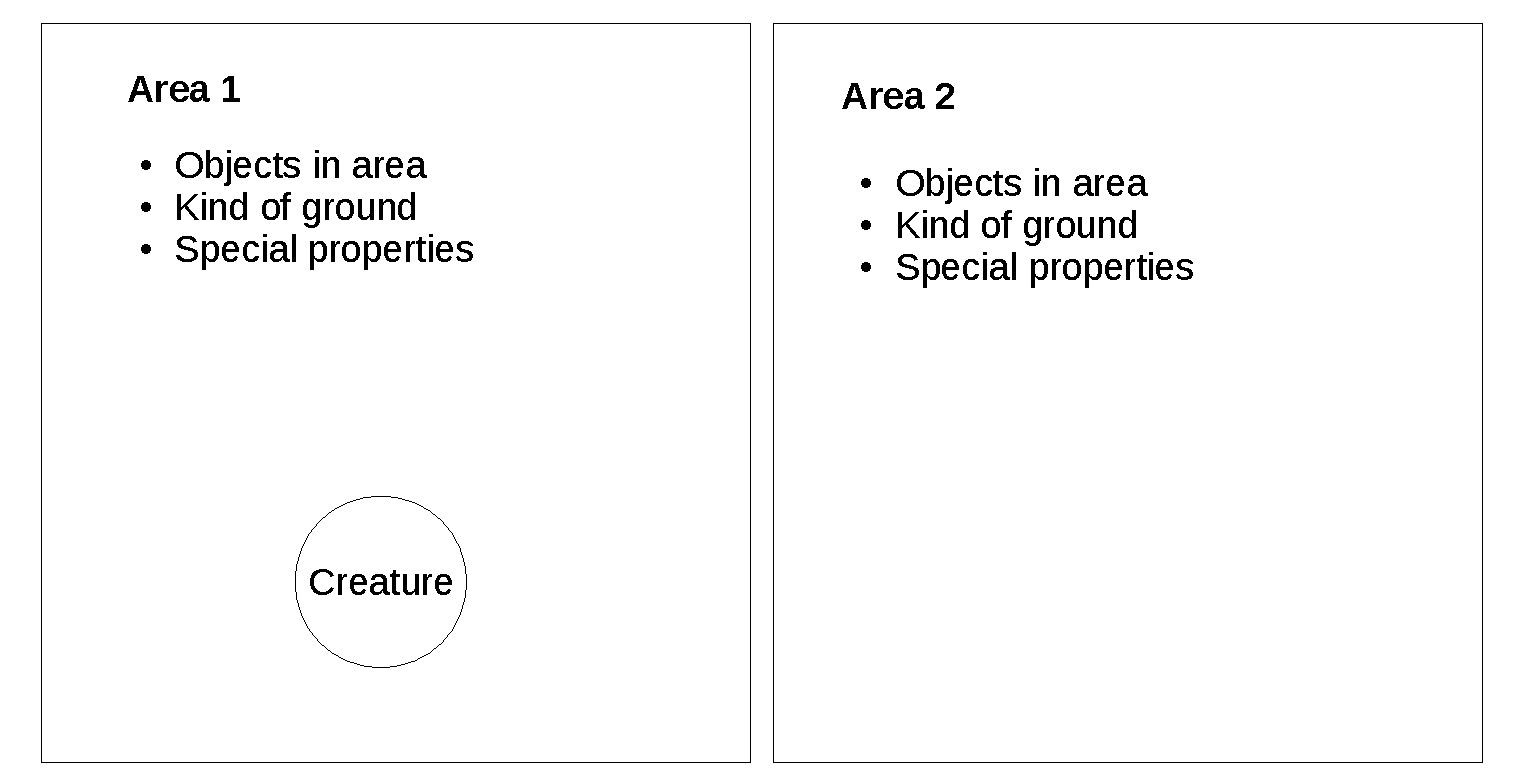
\includegraphics[scale=0.5]{combat0}

\subsection{Combat areas}
In the diagram above we can see a basic schematic of a battle scenario, you can make these out of cardboard for your own games. It consists of two areas, here just called 1 and 2. Each area will obviously have a more descriptive name in an actual fight, and have actual properties detailed on it. The type of terrain should be noted so that players know how hard it is to move around the fight, and whether there are objects or circumstances they can take advantage of (like boulders they push down a hill, or a river they can knock enemies into). Creature tokens can be used to represent which players or enemies are currently in which area. Leaving a combat area that contains enemies results in a \textlf{Moment of weakness} (see Section~\ref{sec:aoo}).

\subsection{Distances and radii}
In this system you measure a distance as the number of area boundaries crossed. So from one area to its neighbour is a distance of 1 (around 15 m). To determine if an enemy is in range of a shooting attack you must count how many area borders the projectile must cross and compare it to the weapon range. 

A radius of 1 would cover a single area and ALL neighbouring areas. An effect that is called \textlfirst{adjacent}, or radius 0, applies to a single combat area, which has a radius of $\sim 5$ m. See Table~\ref{tab:distances} for more details about a default system for distance conversions. You can, of course, adjust the distance scale when considering things like spaceship battles etc. 

\begin{table}[ht!]
	\centering
	\begin{tabular}{|l|l|}
		\hline
		Area distance & True distance \\
		\hline
		0 & < 5 m \\
		1 & 15 m \\
		2 & 25 m \\
		3 & 35 m\\
		\hline
	\end{tabular}
	\caption{Example distance conversions for combat between individual fighters. The distance from one combat area to another is 5 m (radius 0) plus 10 m per area boundary crossed.}
	\label{tab:distances}
\end{table} 

\subsection{Movement}
Most creatures may transfer between combat areas that share a boundary unless otherwise noted or modified by terrain. Movement actions cost 1 action point if the character wishes to change combat area. Normal movement in this manner is thus said to have a range of 1. 

\subsection{Attacks}
Attack-type actions represent making attempts to injure an enemy, they come in two varieties: ranged attacks, which are made with bows, guns, etc., and close-combat attacks which are made with swords, fists, etc. Successful attacks represent breaking through the target's guard and thus grant an opportunity to inflict damage (more on this later). 

Declaring an attack costs 1 action point. During resolution the attacker and their target make an \textlf{opposed roll} with \textlf{aim} and \textlf{deflect} respectively. If the attacker wins, then they gets the opportunity to roll \textlf{damage checks} with the weapons they currently wield.  A character can only make one attack-type action per turn. If an attacker is not \textlf{proficient} with their weapon, they have \textlf{edge-} on \textlf{aim}.

\subsubsection{Penetrating hits} 
If an attacker wins their \textlf{opposed roll} of \textlf{aim} vs \textlf{deflect} by $\dicecritlvl$ or more, then they have achieved a \textlfirst{penetrating hit}. This allows associated \textlf{damage checks} to gain one \textlf{edge+} per \textlf{critical success} threshold. 

\subsubsection{Close-combat}
A character can make close-combat attacks against any creature within the same combat area as they are (range 0).

\subsubsection{Ranged}
A character armed with a ranged weapon can often attack enemies that are in different combat areas to itself. How far it is allowed to do so is defined by the weapon's range score. A range of 1 would allow shots to be fired at a target in any adjacent area to that of the firer. To determine the required range to a target, simply draw a straight line between it and the shooter then count the number of area boundaries it passes over. A ranged weapon can fire a distance up to twice its range score, but receives \textlf{edge-} on \textlf{aim} if doing so.

These weapons are divided into two types: shooting and throwing. Throwing a weapon/object without the \textlf{throw} property incurs \textlf{edge-} on \textlf{aim}. Firing a shooting weapon at a target within range 0 incurs a similar penalty. Unless specially constructed or robust, shooting weapons usually incur \textlf{edge-} on \textlf{aim} when used as close-combat weapons.

\subsubsection{All-out attack}
The character channels all their energy into aggression. This attack action costs 2 action points but grants \textlf{burst} + 1 to the attack (for one of the character's weapons if attacking with two).

\subsubsection{Unarmed attacks}
A character can attack their opponents with fists and feet, or other appendages. Unarmed characters may make a single punch/kick for 1 action point, this fighting style has its own \textlf{weapon proficiency}.

\subsubsection{Multiple weapons}
If the character is using a weapon in each hand, it costs 1 extra action point to make attack-type actions. Only one \textlf{opposed roll} of \textlf{deflect} vs \textlf{aim} is made, but, each weapon gets a separate \textlf{damage check}. If the character wishes to divide their attack between opponents then make separate \textlf{deflect} vs \textlf{aim} checks for each target.

Character's with certain \textlf{perks} (\textlf{Two-weapon mastery perk}) ignore the extra action point cost for attacking with both weapons. If either weapon has a \textlf{reload} rule, the reload time is increased by 1 action point. Finally, a character with \textlf{two-weapon fighting proficiency} may swap two weapons at once for a single action point.

\subsubsection{Attacking objects or huge enemies}
Sometimes you need to attack an inanimate object, like a barn door, or a vast enemy that is easier to hit than a barn door. These targets obviously cannot actively evade your attacks. However, you could still miss or land glancing blows due to the situation or your own incompetence. As such, you make an \textlf{aim} check versus \textlf{difficulty} 7 for an object within 5 m and at least 1 m long in some dimension. Small or moving objects should be more difficult, the GM should choose an appropriate difficulty between 5 (extremely easy, 5\% chance to miss) and 18 (almost impossible). This should also be applied when trying to target small regions of large targets (e.g. eyes). In some cases highly mobile parts of a huge enemy (the head of a giant snake for instance) will still be able to actively \textlf{deflect}.


\subsection{Damage checks}
\label{sec:dmg}
This represents whether or not a telling blow penetrates your target's armour. This is a \textlf{difficulty check} with your \textlf{power} against the victim's \textlf{toughness}. If not \textlf{proficient} with their equipped weapon, the attacker suffers \textlf{edge-} on these checks. If the check succeeds then the victim loses \textlf{endurance} or suffers \textlf{wound} effects.

\subsubsection{Losing endurance}
If the victim of a \textlf{damage check} has remaining \textlf{endurance} then these points will be lost before any \textlf{wounds} are suffered. One \textlf{endurance} is lost per point of the attack's \textlf{lethality} (default is 1). Once a character has no \textlf{endurance} left (minimum is 0), further damage is accumulated as actual injuries which are tracked via \textlf{wound} effects. 

\subsubsection{Wound effects}
A character with 0 \textlf{endurance}, who suffers further damage increments their \textlfirst{wound level} by the attack's \textlf{lethality} score. \textlf{wound levels} are \textlf{wounded} (1), \textlf{badly wounded} (2), \textlf{mortally wounded} (3), and \textlf{dead} (4).

\subsubsection{Critical hits}
If an attacker succeeds on a \textlf{damage check} by $\dicecritlvl$ or more, the attack's \textlf{lethality} is increased by 1 per $\dicecritlvl$ they exceeded the victim's \textlf{toughness} by.

\subsubsection{Restoring endurance}
If a character suffering from \textlf{wounds} has their \textlf{endurance} restored to values $>0$ there is no effect on their \textlf{wounds}, the latter can only be remedied by the \textlf{healing skill} or time.

\subsection{Wound levels}  
Here we detail the effects of each \textlf{wound level}.

\subsubsection{Wounded}
This represents a moderately serious flesh-wound and inflicts \textlf{stunned} on the victim (attack actions cost 1 extra action point) until healed. 

\subsubsection{Badly wounded}
This represents severe injuries that temporarily cripple the character's ability to take decisive action. This results in \textlf{edge-} on all rolls until remedied, in addition to the \textlf{wounded} effects.

\subsubsection{Mortally wounded}
A \textlf{mortally-wounded} character is on the brink of death. They cannot make actions and will die in three days unless they receive some medical attention. This status can only be removed by active healing (you obviously can't wait for it to get better).

\subsubsection{Dead}
Time to make a new character.


\subsection{Armour}
Armour provides protection bonuses in the form of additional \textlf{Toughness}. A character's total is 8 plus armour bonuses. However, protection comes at a price and weighty armour makes certain tasks more difficult, like dodging, climbing, and swimming. 

\subsubsection{Light armour}
This does not have adverse effects on the wearer, as it is light and flexible. 

\subsubsection{Medium armour}
\textlf{Medium Armour} applies \textlf{edge-} to \textlf{Athletics} and \textlf{Stealth}.

\subsubsection{Heavy armour}
\textlf{Heavy Armour} applies \textlf{edge-} to \textlf{Athletics}, \textlf{Stealth}, and \textlf{Deflect}. Characters in \textlf{heavy armour} also have to spend an extra action point to stand up after being \textlf{knocked down}.


\section{Other actions in combat}
There is a lot more you can do in combat than just attack.

\subsection{Anticipate}
A fighter can try and predict their opponent's next move. This costs 1 action point but grants the character a bonus reaction point that lasts until the next round ends.

\subsection{Change weapon}
To swap a currently held weapon a character must spend 1 action point. To swap two wielded weapons it thus costs 2 action points.

\subsection{Defensive stance}
A fighter can assume a defensive posture, ready to fend off attackers. This costs 1 action point. The character gains \textlf{edge+} to \textlf{deflect} the next attack made against them.

\subsection{Disarm}
Even the mightiest warrior can be flummoxed by the loss of their precious sword. 
This is a modified, close-combat attack, replacing a \textlf{damage check} with an \textlf{opposed roll} between yourself and the target using \textlf{wit}. Should you win, the target cannot use their current weapon without either spending 1 action point or suffering a \textlf{moment of weakness} to retrieve it. Weapons with the \textlf{disarming} rule cause damage on a \textlf{critical success}. If your \textlf{disarm} action benefits from two copies of this rule then it deals damage on a \textlf{success} instead.

\subsection{Feint}
\label{sec:feint}
A \textlf{feint} is an attempt to confuse your target, making them think your attack will come from one angle before changing at the last minute. This costs one action point and requires an \textlf{opposed roll} between yourself and the target using \textlf{cunning}. Success allows you \textlf{edge+} to \textlf{aim} this round, while \textlf{critical failure} results in a \textlf{moment of weakness}. This has no effect with ranged weapons unless otherwise modified.

\subsection{Grapple}
You can attempt to wrestle your foe into an immobile state at the cost of 1 action point (provided you have at least one free hand). You and your target make an \textlf{opposed roll} with \textlf{Might}. If you win, the target is now \textlf{grappled}. However, if you score a \textlf{critical failure}, you suffer a \textlf{moment of weakness}. A \textlf{critical success} makes your target lose 1 action point in the next round. It costs 1 action point each round after the first to maintain a grapple.

\textlf{Grappled} creatures cannot make any movement actions until they break free of the \textlf{grapple}, this costs 1 action point and requires that they win a \textlf{might}-based \textlf{opposed roll} with the grappler. If they are forced to move by some external effect then the grapple breaks automatically. All participants have \textlf{edge-} on \textlf{aim} versus each other, unless using \textlf{small} or natural weapons. Creatures not involved in the grapple suffer \textlf{edge-} to hit any participant.

\textit{Designer's note: \textbf{Grapple} is not the same as the \textbf{Immobilised} condition, as it represents a state of active wrestling and thus does not make it easier for other fighters to hit the grappled target}.

\subsection{Prepared actions}
\label{sec:prep}
A \textlfirst{prepared action} is one that the character does not wish to make immediately. Instead, they specify the actions they wish to make and spend action points as normal. In addition, they must specify a condition to trigger the prepared actions. Such as: they will make their actions in response to a specific action made by an enemy, or to an environmental event, like a wall collapsing. Having specified their prepared actions, the character then waits and executes the prepared action when the condition is met (at a cost of 1 reaction point). If the condition is not met by beginning of the next action declaration, then the prepared action is not performed and the fighter may act as normal.

\subsection{Run}
A character can run, at a cost of 2 action points, they then add 1 to their movement range and gain \textlf{edge+} on \textlf{deflect} until the round ends. 

\subsection{Retreat}
This represents a careful withdrawal from active combat, ready to fend off any parting shots. At a cost of two action points the character can make a normal move, while leaving an area occupied by enemies, and not suffer a \textlf{moment of weakness}.

\subsection{Shove}
A fighter can knock a target off their feet or push them away to create space. This costs 1 action point and involves an \textlf{opposed roll} between yourself and the target using \textlf{might}. If the shover is successful, the target is either knocked down or moved into an adjacent combat area (at the shover's discretion). \textlf{critical failure} results in the shoving character experiencing a \textlf{Moment of weakness}. \textlf{critical success} results in the victim suffering a \textlf{damage check}.

\subsection{Taunt}
With cutting words, or obscene gestures, you bait a foe into attacking you. This costs 1 action point and the target must be able to understand the provocation in some way. Make an opposed check with your \textlf{resolve} and the target's \textlf{wit}. If you win, the target now attempts to attack you instead other targets. 

\subsection{Trip}
Attempt to entangle your foe's legs with your weapon's haft, or pointy bit built for tripping. This modifies a close-combat attack: replace a \textlf{damage check} with an \textlf{opposed roll} between yourself and the target using \textlf{cunning}. Should you win, the target is \textlf{knocked down} (see Section~\ref{sec:special}). Weapons with the \textlf{Tripping} rule cause damage on a \textlf{critical success}. If your \textlf{trip} action benefits from two copies of this rule then it deals damage on a \textlf{success} instead.


\section{Reactions in combat}
These are the default reactions available to all combatants. Numerous additional reactions can be acquired by buying \textlf{perks}. 

\subsection{Desperate effort}
This costs 1 reaction point and can be used when the character fails a check in combat (not including \textlf{skill} checks). This allows the character to re-roll the check, they must accept the result of this re-roll. This cannot be used if the character has any \textlf{edge} bonuses on the roll.

\subsection{Exploit weakness}
\label{sec:exploit}
This costs 1 reaction point and can be used when an enemy within range 0 experiences a \textlf{moment of weakness} (see Section~\ref{sec:aoo}). This allows the character to make a single close combat \textlf{damage check} against the enemy. This reaction can only be used once for a single \textlf{moment of weakness}.


\section{Recovery and healing}
\textlf{endurance} is recovered completely if the character can rest for 8 hours. Otherwise, a short rest of around an hour, or a heat meal, restores 1 \textlf{endurance}.

A character that has suffered wounds can be healed via use of the \textlf{Healing skill} or by a non-player healer. Without healing, a character recovers from the \textlf{wounded} effect after 3 days. It takes 7 days before the \textlf{badly-wounded} effect is reduced to \textlf{wounded}.








\section{Combat areas - terrain}
\label{sec:terrain}
\subsection{Open terrain}
Grass, sand, tiles, gentle slopes or terrain that offers otherwise firm-footing is open terrain. This confers no bonuses or penalties to movement over it.

\subsection{Rough terrain}
\label{sec:rough-t}
This includes: loose rocks, tree roots, rubble, tables and chairs, obstructions of about knee or waist height, and surfaces that are unstable/moving/irregular. Moving through \textlf{rough terrain} costs 1 action point more than normal.

For characters riding or driving, moving in \textlf{rough terrain} requires a ride/drive check versus a \textlf{difficulty} (chosen by the GM) between 8 and 12 (depending on how rough the terrain is) to avoid being unseated or losing control. 

\subsection{Dangerous terrain}
Marsh-land, fast-flowing water, quicksand, thin ice, brittle rock, pools of acid or hot mud; these sorts of things are \textlfirst{dangerous terrain}. Any character entering, occupying, or moving through this terrain takes a hit with \textlf{lethality} 2 that causes damage on a $\dicediffbase+$ regardless of \textlf{toughness}. \textlf{Rough terrain} movement restrictions apply here as well.

For characters riding or driving, \textlf{dangerous terrain} requires a riding/driving check versus a \textlf{difficulty} (chosen by the GM) between 11 and 16 to avoid being unseated.



\section{Combat areas - cover}
\label{sec:cover}
If a combat zone offers cover then any creature within the zone may claim a bonus to \textlf{deflect} against attacks made from outside the zone. Cover is divided into three categories and examples will be given below.
\begin{table}[ht]
	\centering
	\caption{Cover table}
	\label{tab:cover}
	\begin{tabular}{|l|l|l|}
		\hline
		Cover type & Deflect bonus & Hide bonus\\ [0.5ex]
		\hline
		Soft & - & \textlf{edge+}\\
		Medium & \textlf{edge+} & \textlf{edge+}\\
		Heavy & \textlf{edge++} & \textlf{edge+}\\
		\hline
	\end{tabular}
\end{table}

\subsection{Soft cover}
Good examples of soft cover are: small trees, bushes, wooden crates, soft furnishings and other such items that provide little protection but may conceal you from your enemies, and so, grant \textlf{edge+} on any rolls to hide in them. Objects that provide soft cover can be broken with a \textlf{might}/\textlf{power} check against \textlf{difficulty} 6-9.

\subsection{Medium cover}
Sandbags, hedges, low walls, small rocks, solid furniture. These kind of things provide a moderate amount of protection and concealment from enemies and \textlf{edge+} to rolls to hide in the cover. Objects that provide medium cover can be broken with a \textlf{might}/\textlf{power} check against \textlf{difficulty} 9-13.

\subsection{Heavy cover}
Battlements, large walls, trees, big rocks, barricades, serious furniture (made of stone or steel). These things are built to provide a lot of cover and protection and also grant \textlf{edge+} to \textlf{hide}. Objects that provide heavy cover can be broken with a \textlf{might}/\textlf{power} check against \textlf{difficulty} 13-20.


\section{Combat areas - examples}

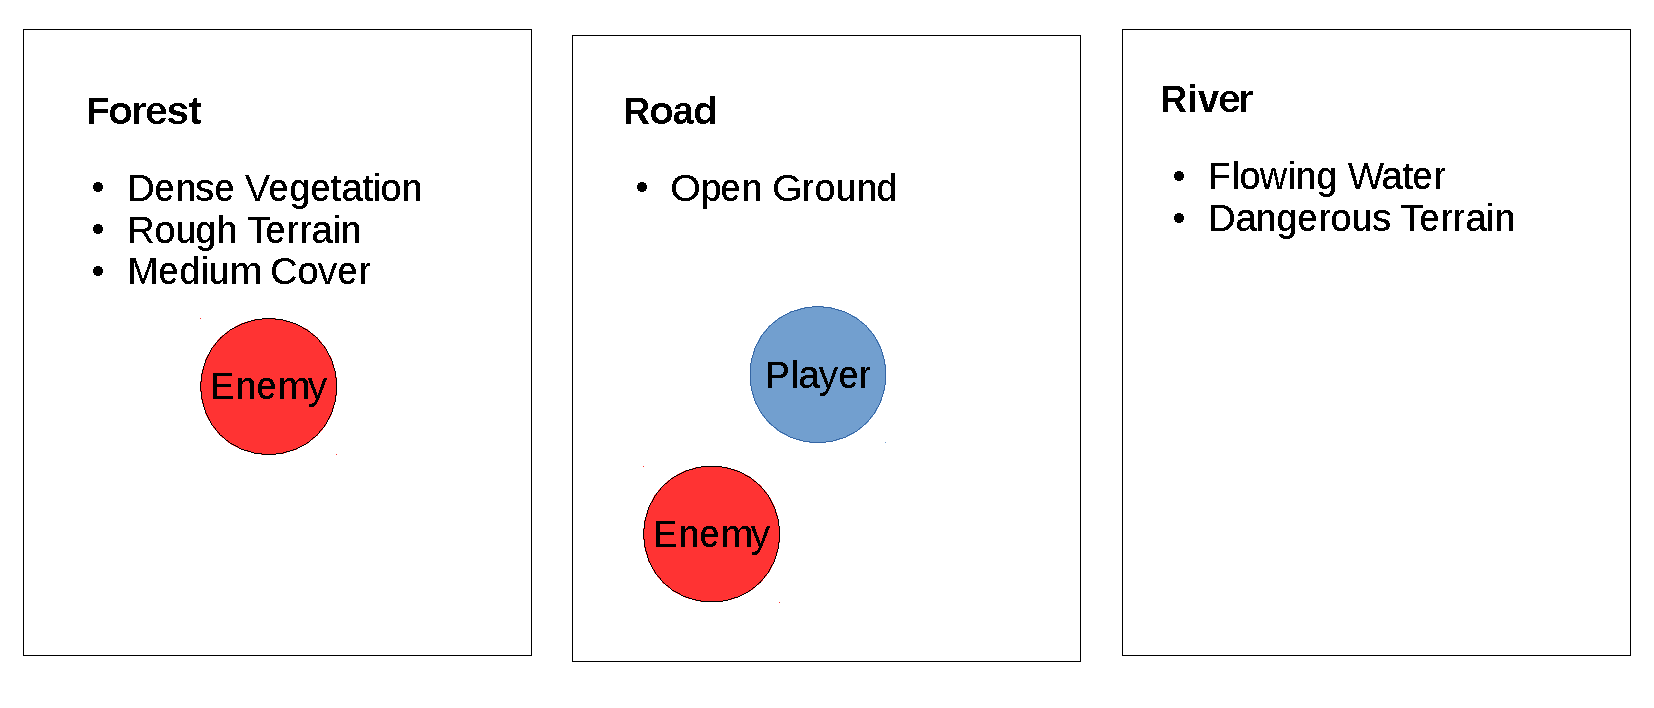
\includegraphics[scale=0.5]{combat1}


In our first example we see a fight with three combat areas. We can see it also has three participants, one player character and two enemies attacking them. The first area is the forest, which is \textlf{rough terrain} and provides \textlf{medium cover}. The road is open ground that confers no effects. Finally, there is a river which is fast-flowing and thus \textlf{dangerous terrain}. We can see that the player and enemy on the road will be able to attack each other with any weapons. While the baddy hiding in the forest will be able to claim a cover bonus but will need a range 1 weapon to strike at the player.


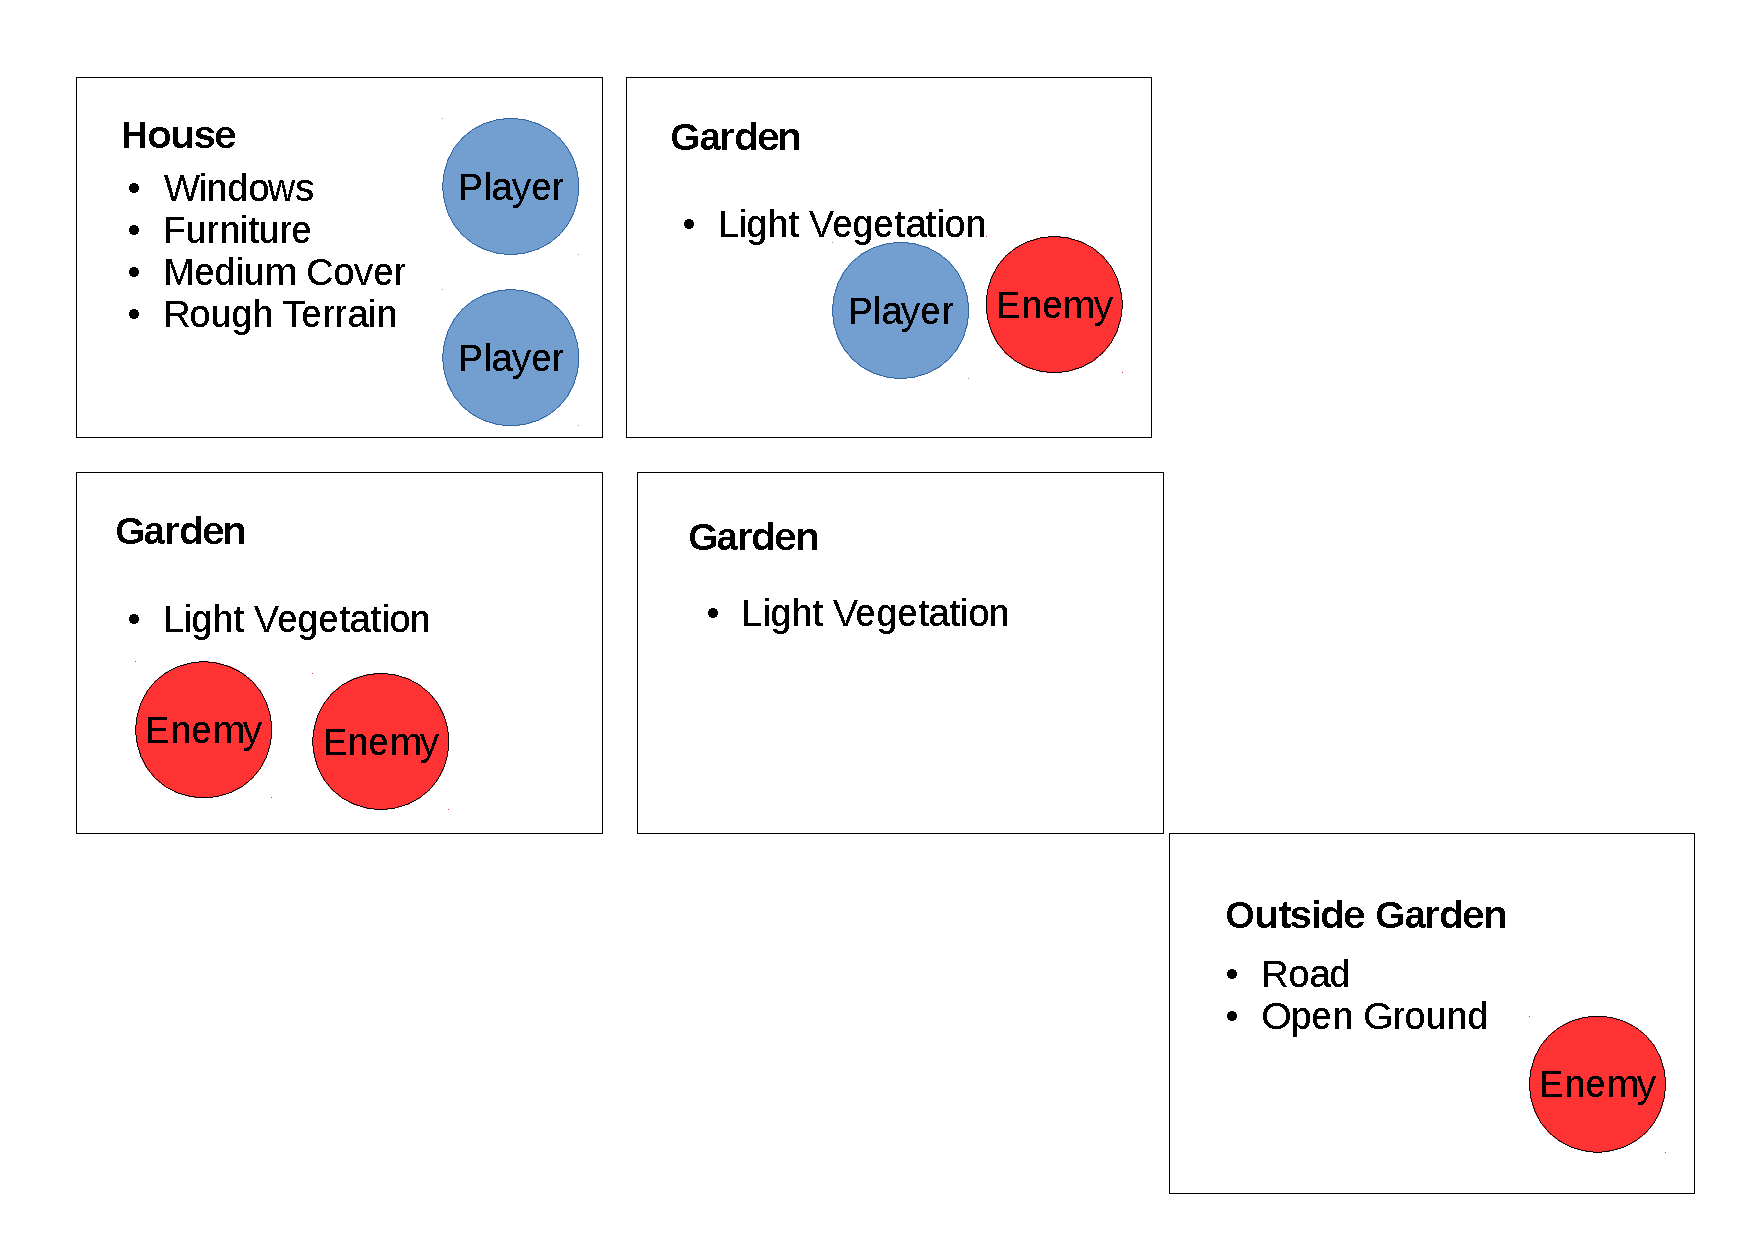
\includegraphics[scale=0.5]{combat2}

Our second example has a far more complex layout consisting of 5 areas. One is a house occupied by two player characters. The house provides medium cover to its occupants and they can attack out of the windows. Additionally, because it is a good defensive position it is labelled \textlf{rough terrain}, so everyone has difficulty moving into/out-of it. The garden has no special effect on combat and neither does the distant road. Players in the house will need range 1 weapons to hit the foes in the garden and range 2 to target the one out on the road. The player and enemy within one garden block can engage in either close-combat or fire ranged weapons at each other.




\section{Situational modifiers}
\label{sec:adv-spc}

\subsection{Light and darkness}
\label{sec:dark}
The lighting of an environment greatly influences the difficulty of fighting within it. There are three types of lighting: \textlfirst{full}, \textlfirst{low}, and \textlfirst{dark}. \textlf{full} lighting has no effect, \textlf{low} incurs \textlf{edge-} on \textlf{aim} and \textlf{awareness}, while \textlf{dark} means the character cannot see at all outside of 5 m (radius 0) and also incurs \textlf{edge--} on \textlf{aim} and \textlf{awareness}.

\subsection{Sneak attacks}
\label{sec:sneak-attk}
A target that does not know of your presence, aggressive intent, or is otherwise fully engaged in combat with someone else (the target must have been unaware of your combat participation, if not your presence) is vulnerable to \textlfirst{sneak attacks}.

The victim of a \textlf{sneak attack} has \textlf{edge--} on \textlf{deflect}.
Such attacks gain \textlf{edge+} to \textlf{damage checks} when made with \textlf{small} weapons, such as daggers, or with specialist tools, such as garrotte wire. Multiple \textlf{perks} can improve \textlf{sneak attacks}. \textlf{Small} weapon bonuses are lost on \textlf{Huge creatures} or larger targets.

\subsection{Rage}
Many cultures hold that great warriors are capable of being consumed by a battle rage. In such condition a warrior is legendarily hard to stop, they can suffer wounds that would kill a normal man and still continue to fight with unbridled savagery. However, this rage makes them reckless, hurling themselves heedlessly into the enemies' ranks.

The mechanics below detail how this berserker fury affects characters and how they can initiate such a state.  

\subsubsection{Becoming enraged}
A character becomes \textlfirst{enraged} if under extreme emotional strain while fighting, although particularly volatile personalities may become \textlf{enraged} more easily. Otherwise a character with the \textlf{Berserker perk} can \textlf{enrage} in the heat of battle.

\subsubsection{When enraged}
An enraged character is immune to \textlf{fear} and \textlf{terror} effects and seeks to enter close combat with the nearest enemy at all times and cannot take prisoners, they go only for the kill. If wielding a firearm-type weapon, they may fire it at range (while moving as required). Enraged characters have \textlf{edge-} on \textlf{deflect} and but \textlf{edge+} on \textlf{damage checks}.

\subsection{Moment of weakness}
\label{sec:aoo}
These are moments when an opponent opens their guard or shows vulnerability, allowing an attacker to strike unhindered. A creature subject to a \textlf{moment of weakness} is open to being targeted by the \textlf{Exploit weakness} reaction~\ref{sec:exploit} which allows a nearby enemy to make a close-combat \textlf{damage check} against them. 

\subsection{Resisting effects}
Some attacks/powers have special effects. These should always be mitigated via \textlfirst{resist(X)}. This involves an \textlf{opposed roll} between the \textlf{power} of the effect and the victim's attribute X. For instance, resisting poison might use \textlf{Resolve}, whereas avoiding being hypnotised would require \textlf{wit}.    





\section{Enemies and monsters}
\label{sec:monsters}
Enemies come in several categories, ranked according to their defining characteristics.

\subsection{Mundane enemies}
These are generally creatures of humanoid or smaller size, this category is largely composed of humanoid soldiers, wolves or similar beasts.
\subsubsection{Abilities and attributes}
Mundane enemies have no \textlf{heroism/villainy}, they can have \textlf{aim} bonuses ranging from -1 to +1, -1 being an inexperienced impromptu fighter and +1 being a well trained soldier. Such foes are likely to have zeros for most attributes, although the more experienced combatants may have one attribute at level 1. The \textlf{endurance} scores of such creatures should be either 0 or 1.
\subsubsection{Tactics}
These enemies are followers, they need to be lead. Without a leader to direct them, they are likely to be easily demoralised by powerful opponents or to simply attack the closest enemy. Such behaviour is over-ridden in the presence of a leader. Mundane enemies suffer the \textlf{panic} effect (see section~\ref{sec:special}) if they lose \textlf{endurance}, suffer a \textlf{wound} effect, or their leader is defeated. Enemies who believe in their cause, or are mindless, have immunity to this. When being lead, a mundane creature may add $1+$ its leader's \textlf{Resolve} score when making \textlf{panic} checks.

\subsection{Elite enemies}
These are generally creatures who are extremely proficient combatants or are enhanced by some magical or technological power.
\subsubsection{Abilities and attributes}
Such fighters are likely to have above average attributes, e.g. two at level 1, with \textlf{aim} of at least $+1$. Elite enemies do not have any heroic attributes but may have multiple combat proficiencies and \textlf{endurance} between 1 and 4. 
\subsubsection{Perks}
Equip these enemies with 1 to 3 \textlf{perks} appropriate to their combat style.
\subsubsection{Tactics}
Such enemies are independent, they do not need to be lead, but are more effective with a leader to direct them. These foes are unlikely to be easily demoralised or intimidated by powerful opposition and will coordinate and work together to defeat stronger opponents. Elites still suffer the \textlf{panic} effect (see section~\ref{sec:special}), but, only if they suffer a \textlf{wound} effect or their leader is defeated. Enemies who believe ardently in their cause, or are \textlf{mindless}, have immunity to this. When being lead, an elite creature may add $1+$ its leader's \textlf{Resolve} score when making \textlf{panic} checks.

\subsection{Enemy leaders}
These are generally creatures who are proficient combatants but are also skilled at directing the actions of underlings.
\subsubsection{Abilities and attributes}
Leader enemies are similar to elites in attributes but also have \textlf{leadership skill proficiency} (and likely a \textlf{resolve} score of 1).
\subsubsection{Perks}
Equip these enemies with 1 to 3 \textlf{perks} appropriate to their combat style.
\subsubsection{Tactics}
Such enemies co-ordinate their allies, using their \textlf{leadership skill} to enhance fighting prowess and allowing lesser allies to adopt more sophisticated tactics. Leaders will attempt to avoid close-combat unless they are heavily reinforced. In other regards they behave similarly to elite enemies.

\subsection{Heroic enemies}
These enemies are powerful heroes, much like the player-characters, except that they oppose the heroes for whatever reason that the GM decides should motivate them.
\subsubsection{Abilities and attributes}
These enemies are individually as capable and powerful as player characters, sometimes more-so, and thus follow the same rules for heroic attributes and determining combat statistic scores. Heroic foes have attributes generated in a similar manner to players, although the Game Master may decide to give them more, or less, attribute points.
\subsubsection{Tactics}
Such enemies are leaders, they direct lesser foes in ways that will maximise their own advantage within a fight, they will also use their heroic attributes to the maximum possible effect. The presence of such enemies inspires and emboldens lesser enemies, making them less susceptible to intimidation and fear ($+1$ to \textlf{panic} checks). Heroic enemies may surrender if they are severely injured or near death but are more likely to try and escape.

\subsection{Monsters}
These are enemies that are usually at least \textlf{large creatures} and often \textlf{huge} or \textlf{titanic creatures} (see Section~\ref{sec:special}). However, enemies that possess incredible supernatural powers or extreme natural abilities might fall into this field as well.
\subsubsection{Abilities and attributes}
Such creatures have access to unique abilities or methods of fighting that might not need to depend on heroic attributes, monsters generally have low \textlf{aim} bonuses, as many monsters are large and have trouble making rapid manoeuvres. However, they have immense strength and aggression, larger creatures having high \textlf{power} to represent this. They may also possess heroic attributes, but this is not needed, they are quite often mighty enough as it is. 
\subsubsection{Tactics}
These enemies are hugely dangerous and will simply exploit the powers, size or strengths that make them monsters in order to win. They attack enemies that seem the easiest prey, or those that otherwise attract their attention, unless they have the opportunity to get more than one foe at once. Some monsters may be extremely stupid, this limited intelligence can be exploited by players to distract or confuse such foes, such monsters may need a handler to direct them and counteract their innate lack of quick wits. Monsters do not know the meaning of surrender or fear.



\section{Universal special rules}
\label{sec:special}
This is a collection of special rules that apply in all campaign settings and always mean the same thing regardless of context.


\subsection{Conditions}
These are negative statuses that a creature can become subject to. 

\subsubsection{Bleeding}
This state represents severe bleeding. It lasts 2 rounds, each round the victim must make an opposed check: their \textlf{resolve} against the \textlf{power} of the effect. Their failure results in the loss of 1 \textlf{endurance} (this does not scale with levels of \textlf{critical failure}). 

\subsubsection{Blind}
A \textlfirst{blind} creature has \textlf{edge--} on both \textlf{aim} and \textlf{deflect} for the effect's duration. In addition, it must randomise direction if it wishes to move.  

\subsubsection{Cursed}
A \textlfirst{cursed} creature is afflicted by a malignant magical effect sapping its luck. \textlf{Critical success} on any roll is reduced by 1 level. \textlf{Curse} lasts until removed.

\subsubsection{Fear}
If a creature is afflicted by \textlfirst{Fear}, they suffer \textlf{edge-} on \textlf{aim} (and all \textlf{skills}) until the effect ends. 

\subsubsection{Immobilised}
An \textlfirst{immobilised} creature cannot move, either due to some magical malaise or due to having suffered damage to its legs. In addition, they suffer \textlf{edge-} on \textlf{deflect}.

\subsubsection{Knocked down}
A creature that is \textlfirst{knocked down} loses its footing and falls over. Such a creature has \textlf{edge-} to \textlf{deflect} close-combat attacks until it can stand up. Standing up can be done only in your own turn. This costs 1 action point. Characters in \textlf{heavy armour} must spend 2 action points.

\subsubsection{Panic}
A creature subject to \textlf{panic} must make a \textlf{resolve} check vs \textlf{difficulty} 10 + missing \textlf{endurance} + a wound score (1 for \textlf{Wounded} etc.). Should it fail, it flees or surrenders, which is up to the Game Master's choice. 

\subsubsection{Poisoned}
Poisoned is a state that results from harmful chemicals being introduced into the victim's system. A poisoned attack that injures a creature, poisons that creature if it fails a \textlf{resolve} check versus a \textlf{difficulty} associated with the virulence of the poison and the size of the dose. A \textlf{poisoned} character has one fewer action point in combat (to a minimum of 1) for 3 days or until cured of the poison. Increase the duration by 1 day per \textlf{critical failure} threshold on the \textlf{resolve} check.

\subsubsection{Staggered}
The shock of injury is a difficult thing to ignore and can incapacitate even the most hardened fighters. A \textlf{staggered} creature loses 1 reaction point. If this reduces a character to negative points, i.e. $-X$, they lose the next $X$ points they would normally gain.

\subsubsection{Stunned}
The sudden shock of a well-placed blow can often neutralise retaliation. If a \textlfirst{stunned} creature attempts to make attacks then these cost 1 more action point than normal.

\subsubsection{Terror}
A character afflicted by \textlfirst{Terror} must run for cover then spend each turn cowering in fear until the effect ends. 

\subsubsection{Vulnerable}
A powerful blow can sometimes open up a fighter to being easily finished off. The next attack directed at the victim benefits from \textlf{edge+} to \textlf{damage checks}.


\subsection{Additional weapon effects}

\subsubsection{Blast X}
(X is an integer) \textlfirst{Blast} weapons explode or fire indiscriminately into a crowd. The attacks of these weapons target an area of radius X (usually 5 + $10\times$ X m). The attacker rolls \textlf{aim} once and each target rolls \textlf{deflect}.

\subsubsection{Burst X}
(X is an integer) \textlfirst{Burst} represents attacks that splash over, or carve into a wide area of flesh. An attack with \textlf{burst} X causes 1 + X \textlf{damage checks} on a successful hit, rather than just one. 

\subsubsection{Cleave X}
(X is an integer) An attack with \textlfirst{cleave} is one that can sweep in great arcs, cutting through many hapless foes with each swing. Such an attack may target up to 1 + X enemies at once. The attacker rolls once with their \textlf{aim} and each defender rolls with their \textlf{deflect}.

\subsubsection{Cumbersome}
Weapons with this rule are either massively heavy or just awkward to manoeuvre. They cost an extra action point to make attacks with.

\subsubsection{Disarming}
Weapons with this rule inflict damage on \textlf{critical success} for the opposed roll in a \textlf{disarm} action. If a weapon attacks gains two copies of this rule, it inflicts damage on \textlf{success} instead.

\subsubsection{Penetration X}
(X is an integer) A weapon with \textlfirst{penetration} is designed to deal with heavily armoured opponents, sliding into weak-points or just inflicting blunt trauma through armour. Attacks from this weapon count the target's \textlf{toughness} as reduced by X, but cannot reduce it below $12$ in this way.

\subsubsection{Reach}
\textlfirst{Reach} represents the ability of close-combat weapons, like pikes, to attack from a longer distance. A character with a \textlf{reach} weapon can make close-combat attacks at range 1. In addition, entering a combat area (5 m radius) containing foes with such weapons incurs a \textlf{Moment of weakness} unless an extra action point is spent when making the \textlf{move}.

\subsubsection{Rending X}
(X is an integer) A well-placed blow from a \textlfirst{rending} weapon rips deep into the target. \textlf{Penetrating} hits from \textlf{rending} weapons have +X \textlf{Power}. 

\subsubsection{Small}
\textlfirst{Small} weapons represent dagger-sized implements. These can used with great speed and easily concealed. Thus, they gain \textlf{edge+} when used as part of \textlf{slight of hand} checks. These weapons also receive additional bonuses during \textlf{sneak attacks} (see Section~\ref{sec:adv-spc}).

\subsubsection{Throw X}
(X is an integer) Weapons with the \textlf{Throw} rule are finely balanced for use as projectiles with range X. Thus, weapons without this rule confer \textlf{edge-} to \textlf{Aim} when thrown (range 1 only). 

\subsubsection{Tripping}
Weapons with this rule inflict damage on \textlf{critical success} for the opposed roll in a \textlf{trip} action. If a weapon attacks gains two copies of this rule, it inflicts damage on \textlf{success} instead.



\subsection{Creature-type rules}

\subsubsection{Small creature}
Diminutive creatures are easily missed, even by the most vigilant of larger things. Consequently they get + 1 \textlf{deflect}. \textlf{small creatures} must be smaller than 1 m in all dimensions.

\subsubsection{Large creature}
A creature is declared large if it is bear-sized or larger (2 m in one dimension and 1 m in other dimensions or 3 m in main dimension). Thus, such creatures can only hide in medium or better cover but gain \textlf{cleave} 2 on all close-combat attacks. A \textlf{large creature} has an innate bonus of +1 \textlf{power}. Such a creature has at least 4 \textlf{endurance} points.

\subsubsection{Huge creature}
Such vast beasts barely notice the damage inflicted by even the largest weapons a man can wield. In consequence they have at least 6 \textlf{endurance} points. Their colossal might means that these creatures also have \textlf{cleave} 3 on all close-combat attacks. \textlf{Huge creatures} have an innate bonus of +2 \textlf{power}. The size threshold to be declared huge is typified by an elephant, 3 m in at least two dimensions or 5 m in the main dimension (height, length, or width depending on monster geometry). 

These creatures are large enough for body areas to take damage independently. Typical division would be 1 region per limb, head, and torso. Such a beast dies if at least 3 body areas are \textlf{Mortally wounded} or if the heart/head/vital-region is destroyed (suffers damage beyond \textlf{Mortally wounded}). 

\subsubsection{Titanic creature}
These behemoths are all but inured to the attacks of normal weaponry. In consequence they have at least 8 \textlf{endurance} points. \textlf{Titanic creatures} have \textlf{cleave} 4 on all close-combat attacks and \textlf{edge+} on \textlf{damage checks} against smaller targets. \textlf{Titanic creatures} have an innate bonus of +3 \textlf{power} and the size threshold to be declared titanic is a requirement of least 10 m in the main dimension or 7 m in at least two dimensions (height, length, or width depending on monster geometry). Such beasts have range 1 on their close-combat attacks. 

These creatures are large enough for body areas to take damage independently. Typical division would be 1 region per limb, head, and torso. Such a beast dies if at least 4 body areas are \textlf{Mortally wounded} or if the heart/head/vital-region is destroyed (suffers damage beyond \textlf{Mortally wounded}).


\subsubsection{Mindless}
\textlfirst{Mindless} creatures have no thoughts, emotions, fear or creativity. Because of this, \textlf{mindless} creatures are immune to many occult powers, as well as the \textlf{fear}, \textlf{terror}, and \textlf{panic} effects. These creatures cannot use any advanced combat rules apart from \textlf{grapple} and \textlf{shove}.







\chapter{Perks}
\label{chap:perks}
These are skills and talents learned or gained by a hero through the course of their adventures. They can be purchased through the expenditure of experience points with their cost given in square brackets. Note that upgrades change their parent \textlf{perk}, they do not occupy a new \textlf{perk} slot.

When you purchase a new \textlf{perk} or \textlf{proficiency}, you must spend 2 hours of down-time practising with your new ability before it can be used in any high pressure situation.

\section{Proficiencies}
These do \textbf{not} occupy equipment slots for passive or active \textlf{perks}, their benefits are always available.

\subsection{Heavy armour [5]}
The character has experience moving and fighting in \textlf{heavy armour}. Thus, they no longer experience \textlf{edge-} on \textlf{deflect} when wearing it.

\subsection{Hero/Villain [0]}
(Requires \textlf{Reputation} level 5) The character has become famous, their praise is much sung, or vile deeds whispered of, in local taverns. The character may increase one \textlf{natural attribute} by 1 point.

\subsection{Instrument proficiency: X [2]}
(Where X is a musical instrument type) The character has learned to play a chosen type of musical instrument (X) and no longer suffers the unknown-instrument penalties when playing this type of instrument.  

\subsection{Language: X [2]}
(X is a language) The character has complete fluency in the chosen language. This increases its cost by 1 each time a character takes it.

\subsection{Skill mastery: X [6]}
(Requires \textlf{Skill proficiency: X}) The character has achieved mastery of their art. Any check for the mastered skill X benefits from \textlf{edge+}. A character can only purchase this once.

\subsection{Skill proficiency: X [2]}
(Where X is a skill) The character is \textlf{proficient} with skill X, see Section~\ref{sec:skill-prof} for details. This increases its cost by 1 each time a character takes it.

\subsection{Two-weapon fighting [2]}
The character may swap two weapons at once for a single action point.

\subsection{Weapon proficiency: X [2]}
The character is \textlf{proficient} in the class of weapons X. Classes should be chosen on similarity of use, e.g. for a medieval setting: swords, bows, daggers, blunt, axes, crossbows, firearms, and pole-arms. One type that is always available is unarmed. If not \textlf{proficient} with a given weapon, the user suffers \textlf{edge-} on \textlf{aim} and \textlf{damage checks}.

%\subsection{Weapon Specialisation: X [6]}
%(Requires \textlf{weapon proficiency: X}) The character has trained long and hard in the use of a particular weapon type (X). As such, they gain \textlf{edge+} on \textlf{aim} when wielding such a weapon. 





\section{Defence}
These \textlf{perks} are oriented towards surviving damage in combat. They must occupy an equipment slot for active/passive \textlf{perks} to be usable.
\label{sec:perks-defence}


\subsection{Evasive [3]}
\textlf{Passive perk}. It's hard to pin you down. This grants the character + 1 \textlf{deflect}, provided they wear \textlf{light armour} or are unarmoured.


\subsection{Fighting retreat [2]}
\textlf{Passive perk}. You are categorically not running away. The retreat action now costs only a single action point.

\subsubsection{Upgrade: Rear-guard action [3]}
(Requires \textlf{Fighting retreat}) And neither are your friends. The benefits of \textlf{Fighting retreat} also apply to all allies adjacent to your character at a cost of 1 reaction point.


\subsection{Hardy [4]}
\textlf{Passive perk}. \textlf{Hardy} characters are mighty and indefatigable, they have an extra point of \textlf{endurance}.


\subsection{Indomitable [3]}
\textlf{Passive perk}. Don't tell me what to do. This allows the character \textlf{edge+} on \textlf{resist} checks against effects that would inflict \textlf{staggered}, \textlf{stunned}, \textlf{immobilised}, or \textlf{knocked-down}.

\subsubsection{Upgrade: Juggernaut [3]}
(Requires \textlf{Indomitable}). Now they are just making you angry. This grants a free movement action after successfully passing a check against an effect that would inflict \textlf{stunned}, \textlf{immobilised}, or \textlf{knocked-down}. This movement cannot trigger a \textlf{moment of weakness}.


\subsection{Interdiction [3]}
\textlf{Active perk}. The character can spend a reaction point when an adjacent ally is hit with an attack, causing the \textlf{damage checks} to be resolved against themselves instead.


\subsection{Reactive defence [4]}
\textlf{Active perk}. The character can spend a reaction point to gain the effect of \textlf{defensive stance} when they are targeted by an attack. 


\subsection{Set to defend [3]}
\textlf{Passive perk}. When the character uses \textlf{defensive stance}, they have \textlf{edge+} on \textlf{deflect} for the next 2 attacks.


\subsection{Sixth sense [2]}
\textlf{Passive perk}. The character is so sharp they can evade even unseen attacks at the very last minute. This allows the character to only suffer \textlf{edge-} on \textlf{deflect} against \textlf{sneak attacks}.


\subsection{True grit [4]}
\textlf{Active perk}. Pain is just information. When the character is reduced to 0 \textlf{endurance} they can spend a reaction point to regain 1 \textlf{endurance}.


\subsection{Your mother was a hamster [2]}
\textlf{Passive perk}. The character has great knowledge of insults and is a master of taunting jibes. \textlf{critical success} on \textlf{taunt} actions means the target is so enraged they suffer from \textlf{edge-} on \textlf{deflect} for 1 round.
\subsubsection{Upgrade: And your father smelled of elderberries [3]}
True mastery achieved. The character has \textlf{edge+} on \textlf{taunt} actions.




\section{Offence}
These \textlf{perks} are oriented towards dealing damage in combat. They must occupy an equipment slot for active/passive \textlf{perks} to be usable.
\label{sec:perks-offence}


\subsection{Adrenaline rush [3]}
\textlf{Active perk}. A surge of adrenaline can grant a fighter great power in times of danger. If the character loses \textlf{endurance} to a \textlf{damage check}, they can spend a reaction point to gain \textlf{edge+} to their next \textlf{damage check}.

\subsubsection{Upgrade: Savage reprisal [3]}
(Requires \textlf{Adrenaline Rush}). Whenever the character triggers \textlf{Adrenaline Rush} they may make a single, free, close-combat \textlf{damage check} against their assailant (provided it is within reach). This attack may also claim the benefit of the bonus granted by \textlf{Adrenaline Rush}. 


\subsection{Aimed shot [5]}
\textlf{Active perk}. This costs two action points and allows the character to make a ranged attack with a single \textlf{damage check} only. This benefits from \textlf{edge+} on \textlf{Aim} and the \textlf{damage check}.


\subsection{Berserker [3]}
\textlf{Active perk}. You mad, bro? The character can quickly be overtaken by the pulse of battle, they can spend a reaction point to \textlf{enrage} if they take or deal any \textlf{wound effects}.

\subsubsection{Upgrade: Berserkergang [3]}
(Requires \textlf{berserker}). The character unleashes their inner fury in a remorseless hail of attacks. When \textlf{enraged}, the character can spend a reaction point to grant \textlf{burst} + 1 to an attack that hits.  

\subsubsection{Upgrade: Seething rage [3]}
(Requires \textlf{berserker}). The character's rage is turns them into a highly focussed killer, inured to all but the worst blows. When \textlf{enraged}, reduce the \textlf{lethality} of any damage suffered by 1, to a minimum of 1.

\subsubsection{Upgrade: Endless rage [3]}
(Requires \textlf{berserker}). The character's rage makes them indefatigable. They gain 1 \textlf{endurance} (up to their usual maximum) if they inflicted any damage in a given turn while \textlf{enraged}.


\subsection{Butcher's blow [3]}
\textlf{Active perk}. The character aims their strikes to inflict maximum trauma. This is an attack action that costs 2 action points. Should the attack cause damage, the target is subject to the \textlf{stunned} and \textlf{staggered} effects in the next round. This effect applies only to creatures a maximum of 1 size category larger than the character.


\subsection{Executioner [3]}
\textlf{Passive perk}. The character has learned to deal death swiftly when the chance arises. As such, when striking an opponent with 0 \textlf{endurance}, the character's attacks gain + 1 \textlf{lethality}. This effect applies only to creatures a maximum of 1 size category larger than the character.


\subsection{Furious assault [4]}
\textlf{Active perk}. A risky manoeuvre, the fighter replaces a considered attack with a hail of furious strikes. When declaring an attack the character may elect it to be a \textlf{furious assault}, granting \textlf{burst} + 1. However, the character suffers \textlf{edge-} to \textlf{aim}. This cannot be used if the weapon requires \textlf{reload} actions.


\subsection{Guard breaker [3]}
\textlf{Active perk}. This attack knocks the foe off balance. The character may declare this special attack for 2 action points. If the attack causes damage then the target suffers \textlf{edge-} on \textlf{deflect} in the next round.


\subsection{Merciless [4]}
\textlf{Passive perk}. The character shows no mercy, dispatching the weak with even greater abandon. \textlf{damage checks} against \textlf{bleeding}, \textlf{knocked down}, or \textlf{stunned} targets gain + 1 \textlf{lethality}.


\subsection{Power attack [4]}
\textlf{Active perk}. Enemy not dying? Just hit it harder! The character can declare a close-combat attack as a ``power attack''. This incurs \textlf{edge-} on \textlf{aim}, but grants \textlf{edge+} to associated \textlf{damage checks}.


\subsection{Reckless attack [4]}
\textlf{Active perk}. The character can declare a close-combat attack to be a ``reckless attack''. This has \textlf{edge+} to \textlf{aim} but the character incurs \textlf{edge-} on \textlf{deflect} for one round.


\subsection{Schadenfreude [4]}
\textlf{Passive perk}. The character gets \textlf{edge+} to \textlf{aim} versus enemies who are subject to any condition (see section~\ref{sec:special}).


\subsection{Splatter [3]}
\textlf{Active perk}. The violence of your blows causes the blood of your foes to stain the soil. This can be used when declaring an attack, the cost is increased by 1 action point. Should the attack cause damage, the target is subject to the \textlf{bleeding} effect.


\subsection{Sweeping strike [3]}
\textlf{Active perk}. The character lashes out around them, striking all too slow to escape. This costs 2 action points and allows the character to make a close-combat attack action that has \textlf{cleave} + 1.

\subsubsection{Upgrade: Whirlwind of steel [2]}
This adds an additional \textlf{cleave} + 1 when using \textlf{Sweeping strike}.


\subsection{The ol' one-two [3]}
\textlf{Active perk}. A close quarters manoeuvre where a quick blow with a fist is used to make room for firing a ranged weapon. This special attack costs 2 action points. Make an unarmed attack, if it hits you may perform \textlf{damage checks} for both the unarmed hit and for a shooting-type, ranged weapon you are wielding. 

\subsubsection{Upgrade: A new one too [2]}
(Requires \textlf{The ol' one-two}). You can make any close-combat attack in place of the required unarmed one. Note that this requires you can still wield the ranged weapon at the same time.



\section{Leadership}
These \textlf{perks} are oriented towards leadership and inspiring allies to greater efforts. They must occupy an equipment slot for active/passive \textlf{perks} to be usable.
\label{sec:perks-leader}

\subsection{At the double! [3]}
\textlf{Active perk} (Requires \textlf{Skill proficiency: leadership}). For 1 action point you grant allies within range 1 (15 m) + 1 movement range this round. 


\subsection{By example [3]}
\textlf{Passive perk} (Requires \textlf{Skill proficiency: leadership}). When you score \textlf{critical success} on a roll, you may inspire an ally this round without spending a reaction point.


\subsection{Decisive leadership [3]}
\textlf{Active perk} (Requires \textlf{Skill proficiency: leadership}). The character can spend a reaction point to use a \textlf{leadership} action at any time during combat.


\subsection{Deeds, not words [3]}
\textlf{Active perk} (Requires \textlf{Skill proficiency: leadership}). Any time the character defeats a foe in combat they may make a leadership action, that would otherwise cost 1 action point, for free. Defeat is defined by the enemy fleeing, surrendering, being incapacitated, or dying. This only triggers if the character's own action resulted in the target's defeat. 


\subsection{Inspiring oratory [4]}
\textlf{Passive perk} (Requires \textlf{Skill proficiency: leadership}). Whenever the character succeeds on a \textlf{leadership} check in combat they can restore 1 \textlf{endurance} to an ally within range 0.


\subsection{Now for wrath! [4]}
\textlf{Active perk} (Requires \textlf{Skill proficiency: leadership}). Spend an action point, and pass a \textlf{leadership} check vs 10, to grant allies, within range 1 (15 m), who target the same enemy as another ally + 1 \textlf{aim}.

\subsubsection{Upgrade: Now for ruin! [3]}
(Requires \textlf{Now for wrath!}). \textlf{Now for wrath!} also grants +1 \textlf{power} to eligible allies. However, the \textlf{difficulty} of the \textlf{leadership} check increases by 2.




\section{Martial arts}
These \textlf{perks} are oriented towards unarmed combat. They must occupy an equipment slot for active/passive \textlf{perks} to be usable.
\label{sec:perks-martial}


\subsection{Extension of self [2]}
\textlf{Passive perk} (Requires \textlf{Weapon proficiency: unarmed}). The best weapon is you. This extends the effects of \textlf{Shatter Strike} and \textlf{Meteor Kick} to a single chosen close-combat weapon type.


\subsection{Iron hand [3]}
\textlf{Active perk}. The character's blows are capable of tossing enemies aside like a child's toys. This is a special attack action that costs of 2 action points. If the attack hits, it inflicts no damage. Instead, the target is knocked flying, up to a distance of range 1 in a chosen direction, while also being subject to a \textlf{knocked-down} state. The victim suffers no damage unless they collide with an obstacle (i.e. enters \textlf{rough terrain} or cover). This effect applies only to creatures a maximum of 1 size category larger than the character.

\subsubsection{Upgrade: Fist of steel [3]} 
(Requires \textlf{Iron-Hand}) As long as the character is unarmed, \textlf{Iron-Hand} attacks inflict damage in the same manner as normal unarmed attacks, in addition to their special effects.


\subsection{Meteor kick [3]}
\textlf{Active perk} (Requires \textlf{Weapon proficiency: unarmed}). The character may make an unarmed attack in the form of a flying kick. This costs 2 action points and the character must move a distance of 1 (ignoring terrain effects) and then make an unarmed attack. Such attacks that succeed on their \textlf{damage check} also inflict \textlf{knocked-down}. The \textlf{knock-down} effect applies only to creatures a maximum of 1 size category larger than the character.


\subsection{Professional wrestling [4]}
\textlf{Passive perk}. The character gains \textlf{edge+} on \textlf{Grapple} and \textlf{Shove} actions.


\subsection{Shatter strike [2]}
\textlf{Active perk} (Requires \textlf{Weapon proficiency: unarmed}). The character gathers all their strength and makes a single unarmed attack, with only a single \textlf{damage check}, at a cost of 2 action points. If this attack causes damage then its victim is \textlf{vulnerable} to the next \textlf{damage check} it suffers.


\subsection{Snake fist [3]}
\textlf{Passive perk} (Requires \textlf{Weapon proficiency: unarmed}). The character has learned to unleash a volley of strikes with hands and feet. Unarmed attacks make an extra \textlf{damage check}. This does not incur \textlf{dual-wielding} penalties.


\subsection{Spontaneous brawler [2]}
\textlf{Passive perk}. This allows the character to treat any weapon or improvised projectile as though it had the \textlf{throw 1} rule. 


\subsection{Take-down [3]}
\textlf{Passive perk}. If you make a \textlf{shove} action against a target you have \textlf{grappled} they are slammed to the ground. This causes the \textlf{shove} to deal damage with \textlf{lethality} 1 in addition to its usual effects. 


\subsection{Third eye [5]}
\textlf{Passive perk} (Requires \textlf{Weapon proficiency: unarmed}). The character gains \textlf{edge+} on \textlf{deflect} while unarmed and wearing at most \textlf{light armour}.


\subsection{Turn the tables [4]}
\textlf{Active perk}. If the character is targeted by a \textlf{grapple} or \textlf{shove} attempt that fails, they can spend a reaction point to successfully use this effect on the grappler/shover. 




\section{Mastery}
These \textlf{perks} are oriented towards utility and skill in combat. They must occupy an equipment slot for active/passive \textlf{perks} to be usable.
\label{sec:perks-mastery}

\subsection{Best offence [3]}
\textlf{Active perk}. Is a good defence. When the character scores \textlf{critical success} on \textlf{deflect}, they may spend a reaction point so that the attacker suffers a \textlf{moment of weakness}. 


\subsection{Bull-headed [2]}
\textlf{Passive perk}. Now the bulls run from you. The character has learned to enter combat with unstoppable momentum. If the character moves in the same turn, or made a \textlf{run} action last round, they have \textlf{edge+} on \textlf{shove} actions (see Section~\ref{sec:adv-spc}) this round. 

\subsubsection{Upgrade: Stampede [2]}
(Requires \textlf{Bull-headed}). The character's \textlf{bull-headed shove} actions may be made against 2 + \textlf{Might} targets at once.

\subsubsection{Upgrade: Trample [3]}  
(Requires \textlf{Bull-headed}). The character may make a \textlf{damage check} against one victim of their successful \textlf{bull-headed shove} actions. 

\subsubsection{Upgrade: Pain train [3]}
(Requires \textlf{Bull-Headed}). Choo! Choo! The character may choose for their \textlf{bull-headed shove} to knock the target(s) flying (distance 1) as well as knocking them down. If a victim hits an obstacle (entering \textlf{rough terrain} or \textlf{cover}) they suffer a \textlf{damage check} with \textlf{power} equal to the character's \textlf{might} and \textlf{lethality} 1.


\subsection{Combat improvisation [5]}
\textlf{Active perk}. When the character hits with a close-combat attack they may spend a reaction point to add a \textlf{trip} or \textlf{disarm} roll (do not sacrifice any \textlf{damage checks}).

\subsubsection{Upgrade: Flourish [2]}
(Requires \textlf{Combat improvisation}). When using \textlf{combat improvisation}, the character's weapon(s) gains the benefit of both \textlf{tripping} and \textlf{disarming} rules.


\subsection{Counter attack [5]}
\textlf{Active perk}. The character may spend a reaction point when they successfully \textlf{deflect} an attack. This allows them to make their own in retaliation (this gains \textlf{edge+} on \textlf{aim} with \textlf{critical success} on \textlf{deflect}).


\subsection{Crusader [4]}
\textlf{Passive perk}. When your ammunition is righteousness you seldom run out. Each time the character defeats an enemy they can regain a point of missing \textlf{endurance}. A defeated enemy is either: killed, knocked out, surrendering, or fleeing. 


\subsection{Duelist [3]}
\textlf{Passive perk}. Elegance, advantage, and a free hand to make sweeping gestures; what's not to love? Fighting with a single weapon only, that does not require two-hands for effective use, allows for much more precise weapon control. Fighting in such a manner grants 1 bonus reaction point each round. Example: fighting with only a single rapier, or a longsword in only one hand (common theme is there is a free hand).

\subsubsection{Upgrade: Buckle your swash [2]}
(Requires \textlf{Duelist}). While fighting with a single weapon (as detailed in \textlf{Duelist}), the character may spend a reaction point to gain \textlf{edge+} to their next \textlf{deflect} after scoring a \textlf{penetrating hit}. 

\subsubsection{Upgrade: Swash their buckle [2]}
(Requires \textlf{Duelist}). While fighting with a single weapon (as detailed in \textlf{Duelist}), the character may spend a reaction point to gain \textlf{edge+} on the next \textlf{aim} roll after they \textlf{deflect} with \textlf{critical success}. 


\subsection{Eagle-eye [2]}
\textlf{Passive perk}. You don't need glasses. The character adds 1 to the range score of all shooting and throwing weapons they employ.


\subsection{Leverage [3]}
\textlf{Passive perk}. \textlf{Trip} and \textlf{disarm} actions also \textlf{stagger} their victims.


\subsection{Plan B [3]}
\textlf{Active perk} (Requires \textlf{Duelist}). Whenever one of the character's attacks is \textlf{deflected}, while in \textlf{Duelist} mode, they may spend a reaction point to draw and throw/fire a \textlf{small} weapon (this doesn't suffer penalties for close range).


\subsection{Sudden feint [2]}
\textlf{passive perk}. The character can spend a reaction point to use the \textlf{feint} action (instead of 1 action point) and does not need to declare this during \textlf{action declaration}.


\subsection{Suppressing fire! [4]}
\textlf{Active perk}. The character fires an indiscriminate volley of projectiles, forcing enemies and allies alike to get their heads down. This costs two action points, the character chooses a target enemy and makes a normal attack action against them. In addition, moving into, through, or out of the target's combat area costs 1 extra action point until the end of the next round. This cannot be used with a weapon that requires action points be spent to reload it between shots. 


\subsection{Two-weapon mastery [8]}
\textlf{Passive perk}. This allows the character to fight with two weapons without paying an extra action point for attack-type actions.


\subsection{Warrior's grace [6]}
\textlf{Passive perk}. The character may attack with \textlf{cumbersome} weapons at the cost of both an action and reaction point (rather than 2 action points). 




\section{Miscellaneous}
These \textlf{perks} don't fit into the other categories. They must occupy an equipment slot for active/passive \textlf{perks} to be usable.
\label{sec:perks-misc}

\subsection{Call in a favour [2]}
\textlf{Passive perk} (Requires \textlf{Background: Silver Spoon}). The character can leverage their social connections to obtain a favour from a local noble, banker, crime-lord, warlord, or oligarch. This \textlf{perk} can only be chosen at character creation. This can only be used once per week.


\subsection{Favoured enemy: X [4]}
\textlf{Passive perk}. Everyone hates something. The character is skilled in the killing of a chosen creature type (X). Against targets of type X  the character has \textlf{edge+} on \textlf{aim}. X must be specific, ``humanoids'' is too broad for instance, but ``humans'' is fine in a cosmopolitan fantasy setting. If the setting is mostly human then ``human'' is still too broad and it must be further narrowed down to a group, ``pirates'' or ``ninjas'' for instance.


\subsection{Favoured environment: X [4]}
\textlf{Passive perk}. The character is skilled at moving and fighting in the chosen environment (X). This grants them \textlf{edge+} to stealth, as well as \textlf{survival} checks while in this setting. The character is also not affected by \textlf{rough} or \textlf{dangerous terrain} associated with this environment.


\subsection{Pack animal [3]}
\textlf{Passive perk} (Requires appropriate background). This \textlf{perk} can only be chosen at character creation. The character brings their hunting companion wherever they go. This grants them  a sympathetic animal companion that understands simple verbal commands and hand signals. The creature must be, at maximum, roughly equivalent to a large dog in size and mass. \textlf{survival} checks can be made to get the animal to perform more complicated actions, like stealing a particular object, or distracting someone's attention. The creature's attributes are species specific. If you are \textlf{proficient} in \textlf{survival}, add 1 to all the combat statistics of your companion. A companion can be replaced, once dead, only at a cost of 5 experience.  The companion has two \textlf{skill proficiencies} chosen from: \textlf{survival}, \textlf{stealth}, \textlf{awareness}, \textlf{Intimidate}, and \textlf{athletics}. 

\begin{table}[ht!]
	\centering
	\begin{tabular}{|l|l|l|l|l|}
		\hline
		Creature & Might & Cunning & Wit & Resolve \\
		\hline
		Canine & 0 & 0 & 0 & 1 \\
		Big cat & 0 & 1 & 0 & 0 \\
		Bird & 0 & 0 & 1 & 0 \\
		Reptile & 1 & 0 & 0 & 0 \\ 
		\hline
	\end{tabular}
\end{table}




\section{Mobility}
These \textlf{perks} are oriented towards movement. They must occupy an equipment slot for active/passive \textlf{perks} to be usable.
\label{sec:perks-movement}

\subsection{Acrobatic movement [3]}
\textlf{Active perk}. Sometimes walking is just too boring. All \textlf{athletics} checks for jumping have \textlf{difficulty} reduced by 2. The character can also spend a reaction point so that their \textlf{move} actions out of, or through, a combat area containing enemies do not incur a \textlf{moment of weakness}. 

\subsubsection{Upgrade: Elegance [2]}
(Requires \textlf{Acrobatic movement}). When using \textlf{Acrobatic movement} the character also ignores all the effects of \textlf{rough} or \textlf{dangerous terrain}.  


\subsection{Hit and run [3]}
\textlf{Active perk}. The character can spend a reaction point after resolving a close-combat attack that hits. This allows them to make a normal move action that cannot trigger a \textlf{moment of weakness}. 


\subsection{Moving target [3]}
\textlf{Passive perk}. When mounted/driving and moving, the character has \textlf{edge+} to \textlf{deflect}.


\subsection{Nimble [3]}
\textlf{Passive perk}. \textlfirst{Nimble} characters are quick and agile. Their movement actions have +1 range while unarmoured or wearing \textlf{light armour}.


\subsection{Quick off the mark [3]}
\textlf{Passive perk}. The character can spend reaction points, in place of action points, to make \textlf{run} actions.




\section{Skills}
These \textlf{perks} are oriented towards enhancing your skills. They must occupy an equipment slot for active/passive \textlf{perks} to be usable.
\label{sec:perks-skills}

\subsection{Last-minute save [3]}
\textlf{Passive perk}. Once per day you can re-roll a skill check if you \textlf{critically fail}.


\subsection{Dramatic arts [2]}
\textlf{Passive perk} (Requires \textlf{Skill proficiency: perform}). You can use \textlf{resolve} rather \textlf{cunning} when using the \textlf{feint} action.

\subsubsection{Upgrade: Virtuoso [4]}
(Requires \textlf{dramatic arts}). Your feint performance is so distracting that it leaves the victim wide open. Allies within range 0 (5 m) gain the benefits of your \textlf{feint} actions.


\subsection{Specialist [3]}
\textlf{Passive perk}. Add + 1 to any rolls with two chosen skills (you must be proficient in them). This can only be chosen once per character.


\subsection{Long practised [5]}
\textlf{Passive perk}. Select a \textlf{skill} you are \textlf{proficient} with and has a \textlf{synergy attribute} score of 0 (you cannot select a \textlf{skill} that is receiving bonuses from other \textlf{passive perks}). You gain + 2 to rolls with this skill. This can only be chosen once per character.




\section{Sneaky tricks}
These \textlf{perks} are oriented towards sneaky tricks in combat. They must occupy an equipment slot for active/passive \textlf{perks} to be usable.
\label{sec:perks-sneaky}

\subsection{Always carry a spare [2]}
\textlf{Active perk} (Requires \textlf{Skill proficiency: perform}). It pays to be prepared. The character can produce a single extra dagger (or other \textlf{small} throwing weapon) in an emergency. This can only be used once per day.


\subsection{Arrow to the knee [2]}
\textlf{Passive perk}. A careful shot to the leg can topple the most stable foes. The character can make \textlf{trip} actions with ranged weapons.
\subsubsection{Upgrade: Knee-capped [2]}
The character counts ranged weapons as having the \textlf{tripping} rule.


\subsection{Blind side [3]}
\textlf{Passive perk}. A deft feint allows the character enough room to fire their ranged weapons against close-combat assailants. When using a ranged weapon against a target within range 0 you may \textlf{feint} as though you were using a close-combat weapon. 


\subsection{Chink in the armour [3]}
\textlf{Active perk}. Close-combat attacks against enemies who are \textlf{knocked down} or \textlf{grappled} gain \textlf{penetration} + 2 at a cost of 1 reaction point.


\subsection{Choose your targets [3]}
\textlf{Passive perk}. The character's \textlf{sneak attacks} versus stationary (not actively moving or in combat) or \textlf{immobilised} targets gain \textlf{penetration} + 2.


\subsection{Cunning plan [5]}
\textlf{Passive perk}. Better than other plans. When making \textlf{sneak attacks}, the character gains a \textlf{power} bonus of 1 plus their \textlf{cunning}.


\subsection{Desperate mechanisms [3]}
\textlf{Active perk}. The character may spend a reaction point to reduce the \textlf{reload} action point costs of ranged weapons by 1. 


\subsection{Kick `em while they're down [4]}
\textlf{Active perk}. For 1 reaction point, attacks this round against \textlf{knocked down} targets become \textlf{sneak attacks}.


\subsection{Low blow [5]}
\textlf{Passive perk}. Uncool, man. The character may also make \textlf{sneak attacks} against enemies who have half or less of their \textlf{endurance} remaining, even if they don't meet any other pre-requisites for \textlf{sneak attacks} (see Section~\ref{sec:sneak-attk}).


\subsection{Lightning fast [4]}
\textlf{Active perk}. The character reacts so quickly that they may seize the initiative for their side at a cost of 1 reaction point and 1 \textlf{heroism}. This effect can only be used during action declaration in combat.

\subsubsection{Upgrade: Swift as death [2]}
(Requires \textlf{Lightning Fast}) The character has \textlf{edge+} on \textlf{aim} and \textlf{damage checks} during a turn when they have triggered \textlf{Lightning fast}.


\subsection{Made you look [4]}
\textlf{Passive perk}. If the character succeeds on a \textlf{feint} action, then their next attack-action against the same target is a \textlf{sneak attack} rather than the normal effects of \textlf{feint}.


\subsection{Now you see me, now you don't [5]} 
\textlf{Active perk} (Requires \textlf{Skill proficiency: stealth}). The character may attempt to use the \textlf{stealth} skill while in combat for 1 action point, fading seamlessly into the background. \textlf{critical failure} results in a \textlf{moment of weakness}. All attacks made after hiding are \textlf{sneak attacks} but reveal the presence of the character. While hidden, the character only incurs \textlf{moment of weakness} penalties due to movement if they are detected.


\subsection{One step ahead [4]}
\textlf{Passive perk}. The character's \textlf{anticipate} actions convert one action point into two reaction points.


\subsection{On the hunt [4]}
\textlf{Active perk}. The character zeros-in on their prey. The character may select a target against which they gain \textlf{edge+} on \textlf{aim} and \textlf{deflect}. However, they suffer a similar penalty against all other targets. A new target may only be nominated once the present target is dead, defeated, or hostilities cease.


\subsection{Pistol whip [3]}
\textlf{Active perk}. When using a ranged weapon that can be wielded in one hand the character may make a ``Pistol Whip''. This is a close-combat attack that knocks the target down if it succeeds in causing damage. If used as part of a \textlf{sneak attack}, the victim must roll \textlf{resist(R)} versus the \textlf{power} of the attack, failure means they are rendered unconscious. These effects apply only to creatures a maximum of 1 size category larger than the character. 


\subsection{Poisoner [2]}
\textlf{Passive perk}. The character has knowledge of poisons and toxins. As such, they can poison a weapon given a few herbs (value 1 d per use). This will inflict \textlf{poison} with \textlf{difficulty} 10 the each time the weapon causes damage within the next hour. It costs 1 action point to apply the poison but it takes 10 minutes to prepare a dose. 

\subsubsection{Upgrade: Skilled poisoner [3]}
(Requires \textlf{Poisoner}) You may add 1 + your \textlf{cunning} to the poison \textlf{difficulty}.

\subsubsection{Upgrade: Master poisoner [3]}
(Requires \textlf{Skilled Poisoner}) The character has suspiciously good knowledge of poisons and toxins. Any poison effects used by the character cause the victim to lose 1 \textlf{endurance} when they fail a \textlf{resolve} check against them.


\subsection{Quick draw [2]}
\textlf{Passive perk}. The character can draw/change a weapon at a cost of 1 reaction point instead of an action point.

\subsubsection{Upgrade: Deceptive draw [4]}
(Requires \textlf{Quick Draw}) The character's attacks, after making a surprise \textlf{Quick Draw} of \textlf{small} weapons are \textlf{sneak attacks}. This bonus cannot be claimed unless the character also changed weapon type (i.e. swapping from a dagger or unarmed to a pistol). %This bonus cannot be claimed if the target is already fighting the character.


\subsection{Too hot to handle [2]}
\textlf{Passive perk}. A precisely placed shot causes the target to drop their weapon. The character can make \textlf{disarm} actions with ranged weapons.

\subsubsection{Upgrade: Underhanded [2]}
The character counts ranged weapons as having the \textlf{disarming} rule.





\chapter{Baggage and encumbrance}
\label{chap:loads}
Even a hero can only carry a limited amount of armour, weaponry, supplies, ladders, ropes, lanterns and the myriad of other things an adventurer might need. The Game Master need not police this too strongly, though don't let it get too silly. Some situations do call for some penalties, such a carrying a heavy pack while wearing heavy armour.

\section{Load penalties}
Carrying too much around can make moving or fighting rather difficult. To reflect this, characters carrying a large back-pack, or wearing heavy armour, suffer \textlf{edge-} to deflect.


\section{Carrying, lifting \& dragging loads}
\label{sec:carry}
A character cannot carry more than a heavy load (20 kg + $5 \times$ \textlf{resolve}) for any real distance, but they can lift up to four times the weight of a heavy load, though only a few inches off the floor. A character can push or drag up to 6 times a heavy load on smooth surfaces, but, on rough or difficult ground, they can push or drag only up to twice a heavy load. A character can lift any load lighter than twice their heavy load limit above their head. However these limits assume the character has lots of time to lift or move the heavy objects. If a character wishes to move or lift something rapidly they must make a \textlf{might} check, the \textlf{difficulty} is given by 8 for objects less than 15 kg, + 1 \textlf{difficulty} per additional 5 kg. If successful, a lifting check like this takes 1 action (3 seconds) to perform. For an object dragged via a \textlf{might} check, the \textlf{difficulty} is given by 8 for objects less than 20 kg, + 1 \textlf{difficulty} per additional 5 kg. Success allows the object to be dragged at the character's movement speed for two action points (6 seconds duration). 



\begin{appendices}

\chapter{Probability distributions}


\begin{figure}[ht!]
	\centering
	\resizebox{0.49\hsize}{!}{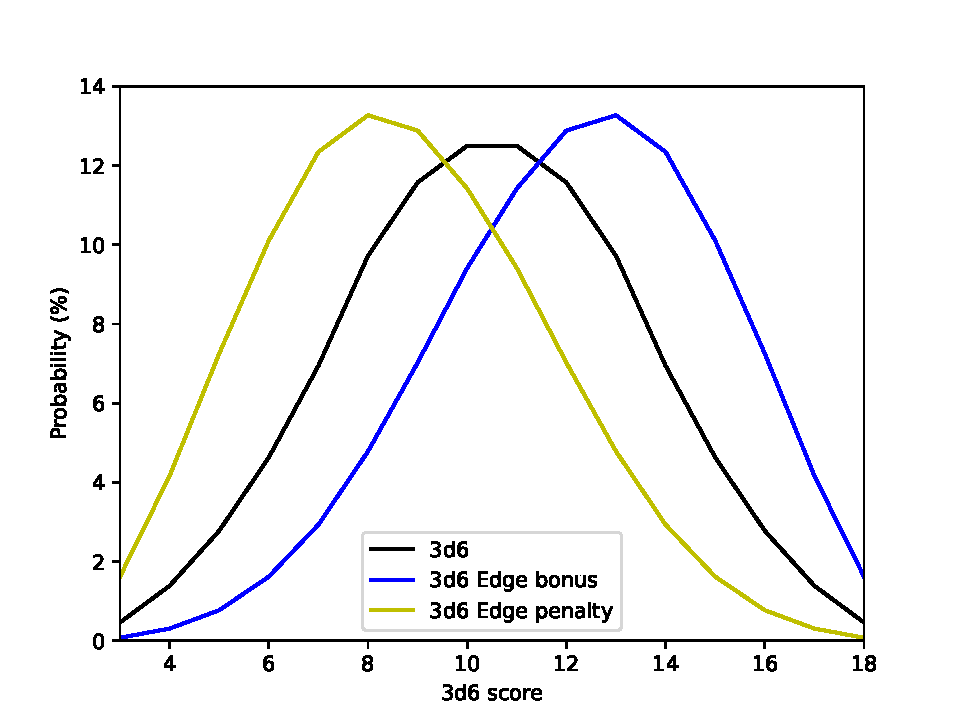
\includegraphics{prob_distribution_3d6.pdf}}
	\resizebox{0.49\hsize}{!}{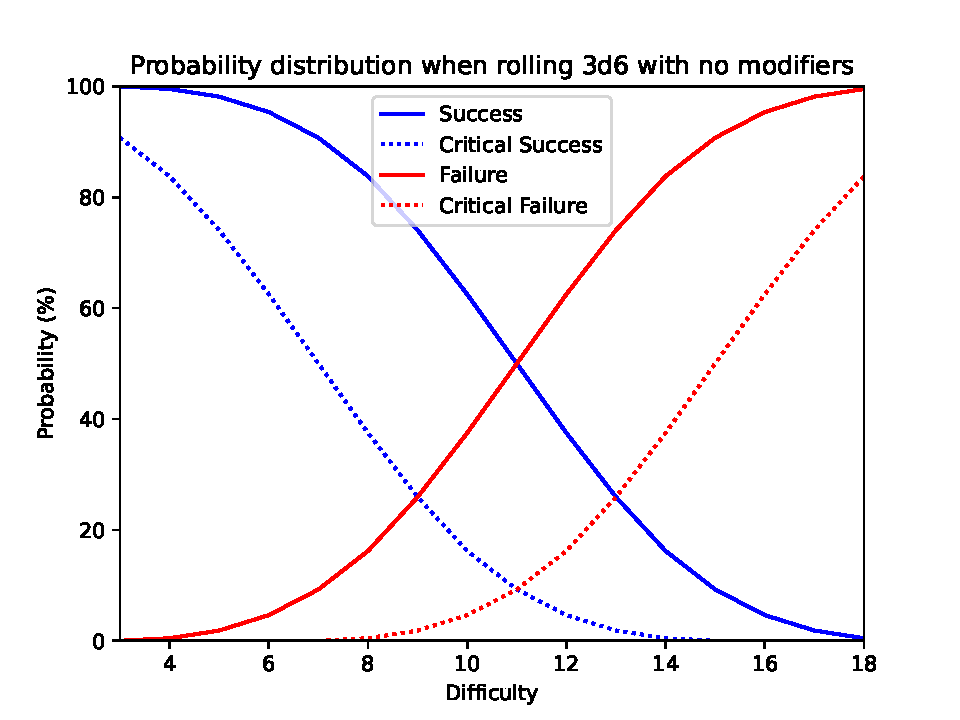
\includegraphics{success_distribution_3d6.pdf}}
	\caption{Left: the probability distribution for scores on 3d6. Right: chances of success and failure for different difficulties on 3d6. } 
\end{figure}

\end{appendices}


\end{document}